\documentclass[usepdftitle=false,aspectratio=169,usenames,dvipsnames]{beamer}
\usepackage{amsmath, amsfonts, amssymb}
\usepackage{xspace}
\usepackage{xparse}
\usepackage[yyyymmdd]{datetime}
\usepackage{ulem}
\usepackage{array}
\usepackage{multirow}
\usepackage{booktabs}
\usepackage{stmaryrd}
\usepackage{subcaption}
\usepackage{bussproofs}
\usepackage{mathpartir}
\usepackage{minted}
% \usemintedstyle{trac}
\usepackage{xcolor}
\usepackage{proof}

\usepackage{tikz}

\usetikzlibrary{shapes,arrows,positioning,decorations.markings,matrix,fit,calc}
\tikzstyle{line} = [draw, -latex']
\tikzstyle{rline} = [draw, latex'-]
\pgfdeclarelayer{background}
\pgfsetlayers{background,main}
\EnableBpAbbreviations


\DeclareUnicodeCharacter{2265}{$\ge$}
\DeclareUnicodeCharacter{2227}{$\wedge$}
\DeclareUnicodeCharacter{2243}{$\simeq$}
\DeclareUnicodeCharacter{2264}{$\mathbb{\le}$}
\DeclareUnicodeCharacter{2200}{$\mathbb{\forall}$}
\DeclareUnicodeCharacter{2228}{$\vee$}
\DeclareUnicodeCharacter{2084}{$_{4}$}
\DeclareUnicodeCharacter{2083}{$_{3}$}
\DeclareUnicodeCharacter{2082}{$_{2}$}
\DeclareUnicodeCharacter{2081}{$_{1}$}
\DeclareUnicodeCharacter{208A}{$_{+}$}
\DeclareUnicodeCharacter{1D62}{$_{i}$}
\DeclareUnicodeCharacter{208B}{$_{-}$}
\DeclareUnicodeCharacter{03B1}{$\alpha$}

\hypersetup{
  pdftitle={Proving Lean theorems via reconstructed SMT proofs}
  pdfauthor={Tomaz Mascarenhas},
  pdfkeywords={},
  pdfborder={0 0 0}
  draft=false,
  bookmarksnumbered,
  bookmarksdepth=2,
  bookmarksopenlevel=2,
  bookmarksopen
}

\renewcommand{\dateseparator}{--}

%%% BEGIN Defining style
\useinnertheme[outline]{chamfered}
\setbeamertemplate{navigation symbols}{}%remove navigation symbols
\usefonttheme[onlymath]{serif}%beamer math looks like article math
\usecolortheme{seahorse}
\setbeamercolor{palette quinary}{use=structure,fg=black,bg=white}
%%% END Defining style

%%% BEGIN Biblatex for references
\usepackage[backend=bibtex,
doi=false,isbn=false,url=false,
% show initials only
style=alphabetic,
% Show name
% style=authoryear-icomp,
% citation label has 4 initials if up to 4 authors, 3 and "+" otherwise
maxalphanames= 4, maxcitenames = 3, minalphanames = 3, minnames = 3]{biblatex}
% citation label has first author's name et al
% maxcitenames=2,backend=biber]{biblatex}

\bibliography{./refs.bib}

%%%%%%%%%%%%% macros

\mathchardef\mhyphen="2D % Define a "math hyphen"

\usepackage{pifont}

\newcommand{\bluecheck}{{\color{blue}\checkmark}}
\newcommand{\greencheck}{{\color{blue}\checkmark}}
\newcommand{\redmark}{\color{red}{\ding{55}}}

\newcommand\vvthinspace{\kern+0.041667em}
\newcommand\vthinspace{\kern+0.083333em}
\newcommand\negvthinspace{\kern-0.083333em}
\newcommand\negvvthinspace{\kern-0.041667em}

\newcommand\FV[1]{\textrm{FV}(#1)}

\newcommand\sym[1]{\mathsf{#1}}

%ADT font macros
\newcommand{\typename}[1]{\mathbf{\mathrm{#1}}}
\newcommand{\consname}[1]{\mathrm{#1}}
\newcommand{\selname}[1]{\mathrm{#1}}
\newcommand{\testername}[1]{\mathrm{#1}}

\newcommand{\SInt}{\typename{Int}}
\newcommand{\SBool}{\typename{Bool}}
\newcommand{\SStr}{\typename{Str}}

\newcommand{\evalfn}[1]{\mathrm{eval}_{#1}}

\DeclareDocumentCommand{\qnt}{ O{n} m O{\psi}}{\innerqnt(#2,#1) #3}
\def\innerqnt(#1,#2,#3){#1 \bar #2.\>}

\DeclareDocumentCommand{\terms}{ m O{}}{\mathbf{T}_{#2}(#1)}

\DeclareDocumentCommand{\bfapp}{ O{f} m O{n}}{#1({\bar #2}_{#3})}
\DeclareDocumentCommand{\enum}{ O{n} m O{,\,} O{} O{1}}{#2_#5#4#3\dots #3#2_{#1}#4}
\DeclareDocumentCommand{\benum}{ O{n} m O{\mapsto} O{} O{,\,} O{1}}{\innerbenum(#2,#3,#6,#4)#5\dots #5\innerbenum(#2,#3,#1,#4)}
\def\innerbenum(#1,#2,#3,#4,#5){#1_{#4}#3 #5{#2_{#4}}}

\DeclareDocumentCommand{\bfenum}{O{\mapsto} m}{\innerbfenum(#2,#1)}
  \def\innerbfenum(#1,#2,#3){\bar #1#3 \bar #2}
\DeclareDocumentCommand{\fapp}{ O{f} m O{n} O{,\,} O{(} O{)}}{#1#5#2_1#4\dots #4#2_{#3}#6}

% Column that takes width (left justified): L{1cm}, e.g.
\newcolumntype{L}[1]{>{\raggedright\arraybackslash$} p{#1} <{$}}

% Column with math mode in displaystyle
\newcolumntype{F}[1]{>{$\displaystyle} #1 <{$}}

% Column with math mode in displaystyle
\newcolumntype{D}[1]{>{\displaystyle} #1 <{}}

% Allows to break like in cell; first arg is $t,b,c$, for alignment with other cells
\newcommand{\specialcell}[2][c]{%
  \begin{tabular}[#1]{@{}l@{}}#2\end{tabular}}

\newcommand{\ccfv}{\textsc{CCFV}}

% \newcommand{\cdclt}{CDCL($\mathcal{T}$)}
\newcommand{\cdclt}{CDCL(T)}
\newcommand{\dpllt}{\cdclt}

\newcommand{\cvcho}{\textsc{cvc}4-\textsc{ho}\xspace}
\newcommand{\cvc}{\textsc{cvc}4\xspace}
\newcommand{\zzz}{Z3}
\newcommand{\verit}{\textsc{veriT}\xspace}

\newcommand{\basestrat}[1]{{\bf #1}}
\newcommand\interleavestrat[2]{\basestrat{#1}+\basestrat{#2}}
\newcommand\mathinterleavestrat[2]{$\mathbf{#1}$+$\mathbf{#2}$}
\newcommand\prioritystrat[2]{\basestrat{#1};\basestrat{#2}}
\newcommand{\zbasestrat}[1]{{\bf z3 #1}}
\newcommand{\zprioritystrat}[2]{{\bf z3} \basestrat{#1};\basestrat{#2}}
\newcommand{\E}{\mathsf{E}}
\newcommand{\Q}{\mathsf{Q}}
\newcommand{\M}{\mathsf{M}}
\newcommand{\ite}{\mathsf{ite}}
\newcommand{\Mod}{\mathcal{M}}
\newcommand{\termordereq}{\preceq}
\newcommand{\termorder}{\prec}
\newcommand{\teq}{\simeq}
\newcommand{\tneq}{\not\simeq}

\newcommand{\inputform}{\psi}
\newcommand{\matrixform}{\varphi}

\newcommand\vitem{\vfill\item}
\newcommand\pvitem{\pause\vfill\item}
\newcommand\pitem{\pause\item}

\newcommand{\cvcsy}{\textsc{cvc}4\textsc{sy}\xspace}
\newcommand{\cvccegis}{\textsc{cvc+c}\xspace}
\newcommand{\cvcu}{\textsc{cvc+upi}\xspace}
\newcommand{\cvcuci}{\textsc{cvc+upi+e}\xspace}
\newcommand{\cvcport}{\textsc{cvc-port}\xspace}
\newcommand{\loopinv}{\textsc{loopinvgen}\xspace}

\newcommand{\divc}{D\&C\xspace}

% AJR : update these
\newcommand{\unif}{Unif+PI\xspace}
\newcommand{\unifci}{Unif+PI+E\xspace}
\newcommand{\smtclass}{\textsc{SMTClassify}\xspace}
\newcommand{\learn}{\textsc{Learn}\xspace}
\newcommand{\classchecker}{\textsc{ClassChecker}\xspace}

%%%%%%%%%%%%


% To avoid number in slides that break, like the references one
\setbeamertemplate{frametitle continuation}{}

% Small font
\renewcommand*{\bibfont}{\scriptsize}
%%% END Biblatex for references



%%% BEGIN DEFINING TITLE PAGE

\defbeamertemplate{title page}{mystyle}[1][]
{
  \vbox{}
  \vfill
  \begingroup
    \centering
    {\usebeamercolor[fg]{titlegraphic}\inserttitlegraphic\par}
    \vskip1em
    \begin{beamercolorbox}[sep=0pt,center,#1,rounded=true,wd=10cm]{title}
      \usebeamerfont{title}\inserttitle\par%
      \ifx\insertsubtitle\@empty%
      \else%
        \vskip0.25em%
        {\usebeamerfont{subtitle}\usebeamercolor[fg]{subtitle}\insertsubtitle\par}%
      \fi%
    \end{beamercolorbox}%
    \vskip1em\par
    \begin{beamercolorbox}[sep=8pt,center,#1]{author}
      \usebeamerfont{author}\insertauthor
    \end{beamercolorbox}
    \begin{beamercolorbox}[sep=8pt,center,#1]{institute}
      \usebeamerfont{institute}\insertinstitute
    \end{beamercolorbox}
    \begin{beamercolorbox}[sep=0pt,center,#1]{date}
      \usebeamerfont{date}\insertdate
    \end{beamercolorbox}%
  \endgroup
  \vfill
}

\setbeamertemplate{title page}[mystyle]

%%% END DEFINING TITLE PAGE

%%% BEGIN Meta information
\author[Tomaz Mascarenhas]
{%
  \texorpdfstring{
    Tomaz Mascarenhas\\Advisor: Haniel Barbosa\\
      \vspace{3ex}
    \begin{columns}
      \column{.45\linewidth}
        \centering
        
\includegraphics[height=0.25\textheight]{images/DCC_LOGO.jpg}
      \column{.35\linewidth}
        
\includegraphics[height=0.15\textheight]{images/Logo_UFMG.jpg}
        % \vspace{2ex}
      %   \centering
      %   
\includegraphics[height=0.15\textheight]{images/DCC_LOGO.jpg}
    \end{columns}
  }
  {}
}

\date{Belo Horizonte, Brazil, 2023/09/12}

\title[Proving Lean theorems via reconstructed SMT proofs]{Proving Lean theorems via reconstructed\\SMT proofs}

% Redifining footer
\makeatother
\setbeamertemplate{footline}
{
  \leavevmode%
  \hbox{%
    \begin{beamercolorbox}[wd=.6\paperwidth,ht=2.5ex,dp=1ex,left]{title in head/foot}%
      {\hspace{1em}\usebeamerfont{title in head/foot}\insertshorttitle}
    \end{beamercolorbox}%
    \begin{beamercolorbox}[wd=.2\paperwidth,ht=2.5ex,dp=1ex,left]{title in head/foot}%
      {\hspace{1em}\usebeamerfont{title in head/foot}Tomaz Mascarenhas, UFMG}
    \end{beamercolorbox}%
    \begin{beamercolorbox}[wd=.2\paperwidth,ht=2.5ex,dp=1ex,right]{title in head/foot}%
      \insertframenumber{} / \inserttotalframenumber\hspace{1em}
    \end{beamercolorbox}}%
  \vskip0pt%
}
\makeatletter
%%% END Meta information

%%% BEGIN Tikz setup
\usepackage{tikz}
\usetikzlibrary{positioning,calc,intersections,backgrounds, fadings}
\usetikzlibrary{shapes}

  \tikzset{
    invisible/.style={opacity=0},
    visible on/.style={alt=#1{}{invisible}},
    alt/.code args={<#1>#2#3}{%
      \alt<#1>{\pgfkeysalso{#2}}{\pgfkeysalso{#3}} % \pgfkeysalso doesn't change the path
    },
  }

\definecolor{BloodRed}{rgb}{.86,0,0}
\definecolor{gold(metallic)}{rgb}{0.83, 0.69, 0.22}

\definecolor{procColor}{rgb}{0.628,0.35,0.17}
\definecolor{cnfColor}{rgb}{0.82, 0.0, 0.86}
% \definecolor{cnfColor}{rgb}{.83,.66,0}
\definecolor{satColor}{rgb}{.83,0,0}
\definecolor{thSolverColor}{rgb}{0,.5,0}
\definecolor{thRwColor}{rgb}{0,0,1}
\definecolor{thCombColor}{rgb}{0.5,0.5,0}

% spec
\definecolor{spec}{rgb}{0.0, 0.0, 0.86}
% syntax recstrictions
\definecolor{grammar}{rgb}{0.82, 0.0, 0.86}

\tikzfading[
  name=arrowfading,
  top color=transparent!0,
  bottom color=transparent!95
]
\newcommand*{\tikzarrow}[2]{%
  \tikz[
    baseline=(A.base),             % Set baseline to the baseline of node content
    font=\footnotesize\sffamily    % Set fontsize of the node content
  ]
  \node[
    single arrow,                  % Shape of the node
    single arrow head extend=4pt,  % Actual width of arrow head
    single arrow tip angle=150,    % Adjust arrow tip angle
    shape border rotate=270,       % Rotate the arrow shape to point down
    draw=red!25,                   % Draw the node shape (with certain border color
    inner sep=2pt,                 % Separation between node content and node shape
    top color=white,               % Shading color on top of node
    bottom color=#1,               % Shading color on bottom of node
    general shadow={               % Specifications for the shadow
      fill=black,
      shadow yshift=-0.5ex,
      path fading=arrowfading
    }
  ] (A) {#2};%
}

%%% END Tikz setup

\newcommand{\qgo}[1]{\innerqgo(#1)}
    \def\innerqgo(#1,#2,#3){#1 #2_1\dots #2_n.~{#3}}
\def\qg#1{\innerqg(#1)}
    \def\innerqg(#1,#2,#3){#1\mathbf{#2}.~{#3}}
\DeclareDocumentCommand{\qgb}{ m O{} }{\innerqgb(#1,#2)}
\def\innerqgb(#1,#2,#3,#4){#1\bar #2_{#4}.~{#3}}
\DeclareDocumentCommand{\fapp}{ O{f} m O{n} O{,} O{(} O{)}}{#1#5#2_1#4\dots #4#2_{#3}#6}
\DeclareDocumentCommand{\fappint}{ O{f} m O{n} O{,}}{\innerfappint(#1,#2,#3,#4)}
  \def\innerfappint(#1,#2,#3,#4,#5,#6){#1(#3#2_1#4#6\dots #6#3#2_{#5}#4)}
\DeclareDocumentCommand{\bfapp}{ O{f} m O{}}{#1(\bar {#2}_{#3})}

\DeclareDocumentCommand{\enum}{ O{n} m O{,} O{} O{1}}{#2_#5#4#3\dots #3#2_{#1}#4}
\DeclareDocumentCommand{\benum}{ O{n} m O{\mapsto} O{} O{,\,} O{1}}{\innerbenum(#2,#3,#6,#4)#5\dots #5\innerbenum(#2,#3,#1,#4)}
  \def\innerbenum(#1,#2,#3,#4,#5){#1_{#4}#5#3 {#2_{#4}}#5}

\usepackage{soul,xcolor}

\setstcolor{red}
\makeatletter
\newcommand\SoulColor{%
  \let\set@color\beamerorig@set@color
  \let\reset@color\beamerorig@reset@color}
\makeatother

\DeclareDocumentCommand{\soutthick}{ O{.4pt} m }{%
    \renewcommand{\ULthickness}{#1}%
       \sout{#2}%
    \renewcommand{\ULthickness}{.4pt}% Resetting to ulem default
}

\definecolor{ao}{rgb}{0.0, 0.0, 1.0}
\definecolor{ao(english)}{rgb}{0.0, 0.5, 0.0}
\definecolor{asparagus}{rgb}{0.53, 0.66, 0.42}
\definecolor{bostonuniversityred}{rgb}{0.8, 0.0, 0.0}
\definecolor{darkbrown}{rgb}{0.4, 0.26, 0.13}
\definecolor{alizarin}{rgb}{0.82, 0.1, 0.26}
% 2952bfff
\definecolor{ceruleanblue}{rgb}{0.16, 0.32, 0.75}
% 8c008cff
\definecolor{darkmagenta}{rgb}{0.55, 0.0, 0.55}
% #8FBC8F
\definecolor{darkseagreen}{rgb}{0.56, 0.74, 0.56}

\usepackage{tikz-qtree}

%%%%%%%%%%%%%%%% BEGIN define outline machinery

\newcommand{\beamersec}[2]{%
  \section*{#1}
  \addcontentsline{toc}{section}{$\bullet$ #1 \vspace{10pt}\newline  \includegraphics[height=.3\textheight]{#2}\vfill}

  \begin{frame}
    \vfill
    \begin{center}
      \vfill\textbf{#1}\vfill
      \includegraphics[height=.5\textheight]{#2}
      \vfill
    \end{center}
    \vfill
  \end{frame}
}

\newcommand{\beamersubsec}[1]{%
  \subsection*{#1}
  \addcontentsline{toc}{section}{$\mbox{}\quad-$ #1 \vspace{10pt}\newline\vfill}

  \begin{frame}
    \vfill
    \begin{center}
      \textbf{#1}
    \end{center}
    \vfill
  \end{frame}
}

\newcommand{\beamersubsubsec}[1]{%
  \subsection*{#1}
  \addcontentsline{toc}{section}{$\mbox{}\qquad\cdot$ #1 \vspace{10pt}\newline\vfill}
}

%%%%%%%%%%%%%%%% END define outline machinery

%%% BEGIN trick for not counting references

\newcommand{\backupbegin}{
   \newcounter{framenumberappendix}
   \setcounter{framenumberappendix}{\value{framenumber}}
}
\newcommand{\backupend}{
   \addtocounter{framenumberappendix}{-\value{framenumber}}
   \addtocounter{framenumber}{\value{framenumberappendix}}
}

%%% END trick for not counting references

\newcommand{\red}[1]{\textcolor{red}{#1}}

% Creating boxes with width of given text; first parameter (optional) is
% alignment of box, then text to be taken the width, then the text to be boxed
\newlength\stextwidth
\newcommand\makesamewidth[3][c]{%
  \settowidth{\stextwidth}{#2}%
  \makebox[\stextwidth][#1]{#3}%
}

% color highlight
% f0dc9cff

\AtBeginSection[]{
  {
    \setbeamertemplate{footline}{}
  \begin{frame}
  \vfill
  \centering
  \begin{beamercolorbox}[sep=8pt,center,shadow=true,rounded=true]{title}
    \usebeamerfont{title}\insertsectionhead\par%
  \end{beamercolorbox}
  \vfill
\end{frame}
}
\addtocounter{framenumber}{-1}
}

% Theorem settings
\addtobeamertemplate{theorem begin}{%
  \setbeamercolor{block title}{fg=white,bg=black}%
  \setbeamercolor{block body}{fg=black, bg=white!90!black}%
}{}

%%% BEGIN CHANGING BULLETS STYLE

\setbeamertemplate{itemize item}{$\vartriangleright$}
\setbeamertemplate{itemize subitem}{$\blacktriangleright$}
\newlength\origleftmargini
\setlength\origleftmargini\leftmargini
\newlength\origleftmarginii
\setlength\origleftmarginii\leftmarginii
\setlength\leftmargini{1em}
\setlength\leftmarginii{1.25em}
\setlength\leftmarginiii{1em}

%%% END CHANGING BULLETS STYLE

\setbeamersize{text margin left=1em, text margin right=1.5em}

\newcommand{\yell}[1]{{\textcolor{red}{[#1]}}}

\newcommand{\cvcc}{\textsc{cvc}{\small 4}\textsc{sy}\textsc{+b}\xspace}
\newcommand{\cvca}{\textsc{cvc}{\small 4}\textsc{sy}\textsc{+u}\xspace}
\newcommand{\gpid}{\textsc{GPiD}\xspace}
\newcommand{\explain}{\textsc{Explain}\xspace}

\newcommand{\mysetminusD}{\hbox{\tikz{\draw[line width=0.6pt,line cap=round] (3pt,0) -- (0,6pt);}}}
\newcommand{\mysetminusT}{\mysetminusD}
\newcommand{\mysetminusS}{\hbox{\tikz{\draw[line width=0.45pt,line cap=round] (2pt,0) -- (0,4pt);}}}
\newcommand{\mysetminusSS}{\hbox{\tikz{\draw[line width=0.4pt,line cap=round] (1.5pt,0) -- (0,3pt);}}}

\newcommand{\mysetminus}{\mathbin{\mathchoice{\mysetminusD}{\mysetminusT}{\mysetminusS}{\mysetminusSS}}}

\def\vv{\smallskip}

\newcommand{\sep}{~\mid~}

\makeatletter
\newcommand\notsotiny{\@setfontsize\notsotiny{7}{8}}
\makeatother

\newcommand\chighlight[2]{\setlength{\fboxsep}{0pt}\colorbox{#1}{#2\strut}}

\begin{document}

{
\setbeamertemplate{footline}{}
\frame{\titlepage}
}
\addtocounter{framenumber}{-1}

\begin{frame}
  \frametitle{History: Computers and Proofs}
  \begin{itemize}
    \item Given a map, what is the minimum number of colors necessary to paint each region in a way that no two adjacent regions share the same color?
    \vitem Conjecture: it is always possible to find such a coloring with at most 4 colors
    \vitem \emph{Four color theorem}: the first major cooperation between humans and computers to prove a theorem
  \end{itemize}
  \centering
  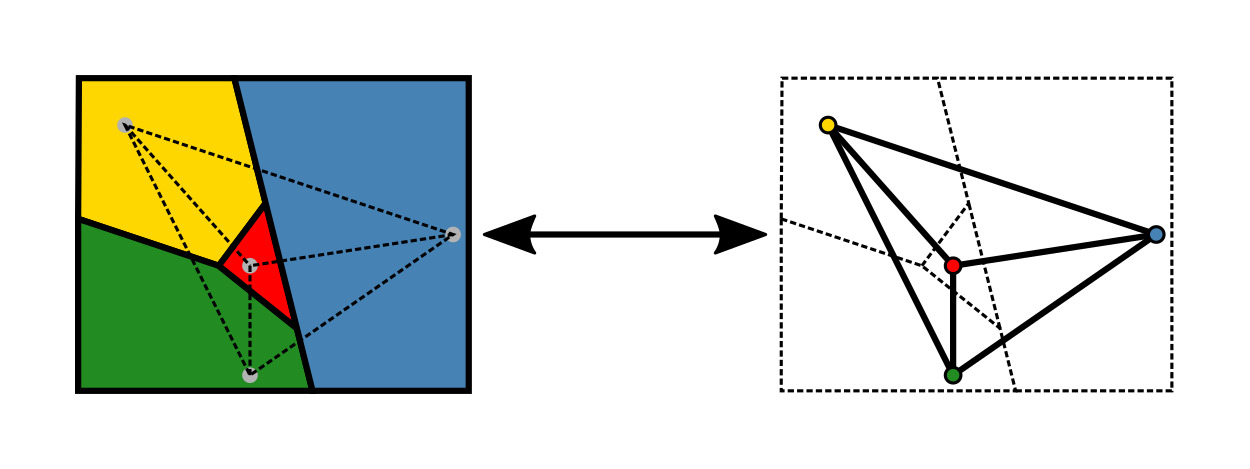
\includegraphics[scale=0.7]{images/fourColor.jpg}
\end{frame}

\begin{frame}
  \frametitle{Automatic and Interactive Theorem Provers}

  \begin{itemize}
    \item Nowadays we have more sophisticated tools that promote the cooperation between humans and computers to prove theorems
    \vitem Interactive Theorem Provers (ITPs) (or proof assistants)
    \begin{itemize}
      \item Proof production guided by the user
      \item Formalization of mathematics
      \item Twelf, Coq, Isabelle, \textbf{Lean}
    \end{itemize}
    \vitem Automatic Theorem Provers (ATPs)
    \begin{itemize}
      \item Define a conjecture and press a button to check its validity
      \item Backend of many systems for verification of software
      \item SMT Solvers (z3, \textbf{cvc5})
    \end{itemize}
  \end{itemize}
\end{frame}

\begin{frame}
  \frametitle{Automatic and Interactive Theorem Provers}
  \begin{table}[]
  \begin{tabular}{|c|c|c|}
  \hline
              & \textbf{Lean}                                & \textbf{cvc5}                          \\ \hline
  Trusted Base & Small kernel                        & Complete software             \\
  Usage        & Build proofs step by step           & Fully automatic               \\
  Expressivity & Calculus of Inductive Constructions & First Order Logic \\ \hline
  \end{tabular}
  \end{table}
\end{frame}


\begin{frame}
  \frametitle{Automatic and Interactive Theorem Provers}
  \begin{itemize}
    \item Cooperation between ATPs and ITPs via proof certificates
    \vitem Hammers: using ATPs to prove theorems stated in the ITP
    \vitem SMTCoq, Sledgehammer (smt tactic)
    \vitem Lean?
  \end{itemize}
\end{frame}

\begin{frame}
  \frametitle{Implementing Hammers}
  \begin{minipage}[c][0.55 \textheight]{0.45 \textwidth}
    \begin{itemize}
      \item Translation Module
      \vitem Premise Selection Module
      \vitem Proof Reconstruction Module
      \begin{itemize}
        \item{Certified vs Certifying}
      \end{itemize}
    \end{itemize}
  \end{minipage}
  \begin{minipage}{0.44 \textwidth}
    \centering
    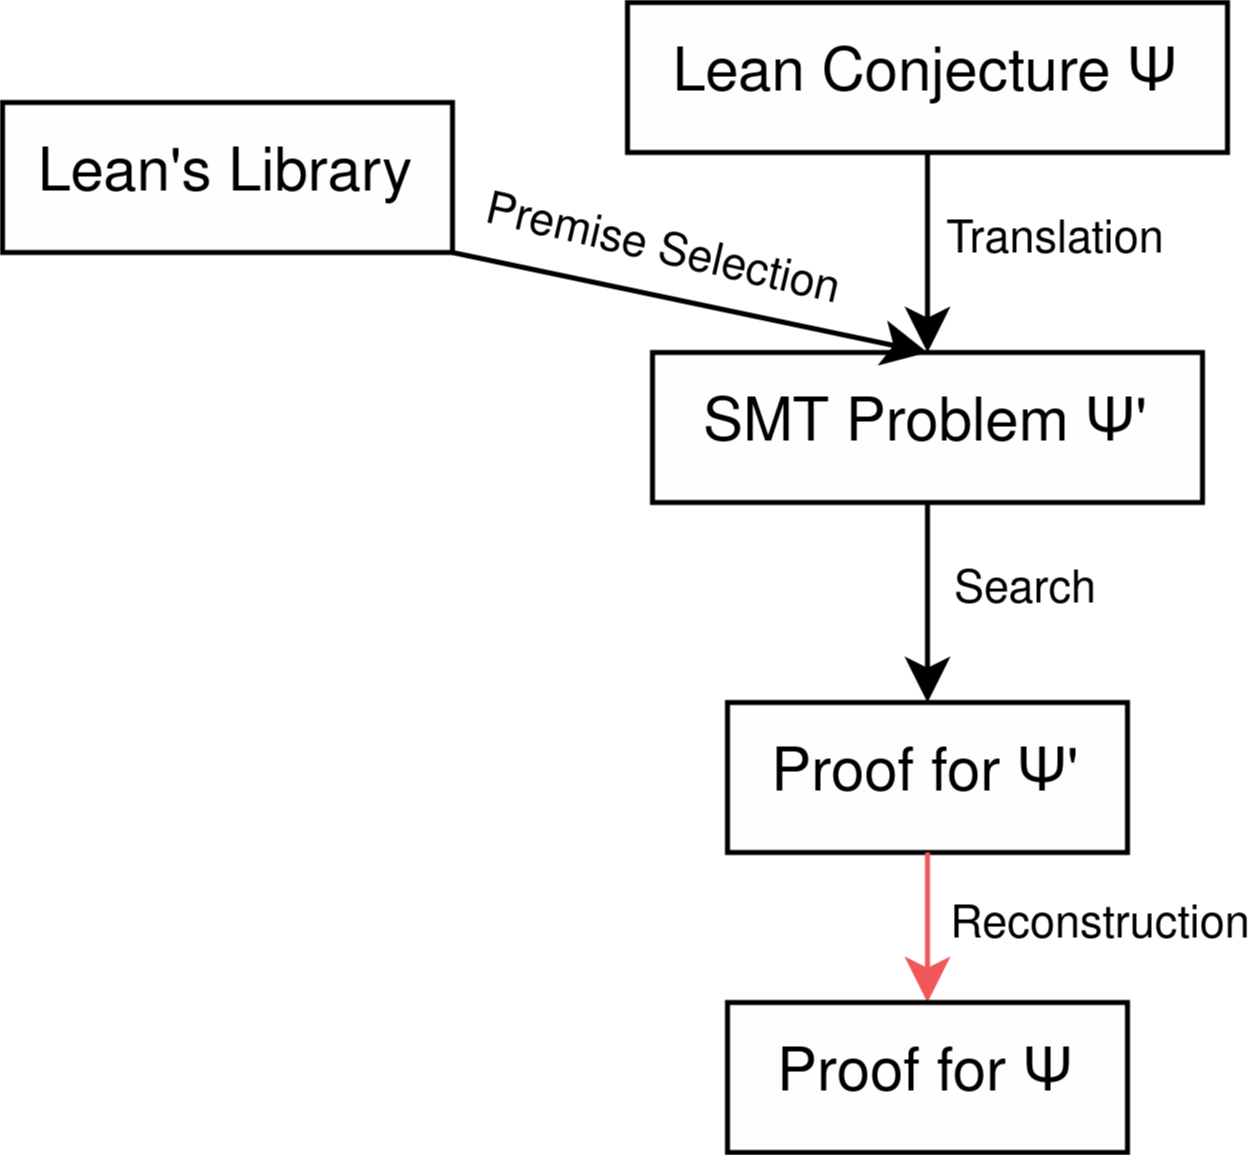
\includegraphics[height=0.65\textheight]{images/pic5.png}
  \end{minipage}
\end{frame}

% \begin{frame}
%   \frametitle{Implementing Hammers}
%   \centering
%   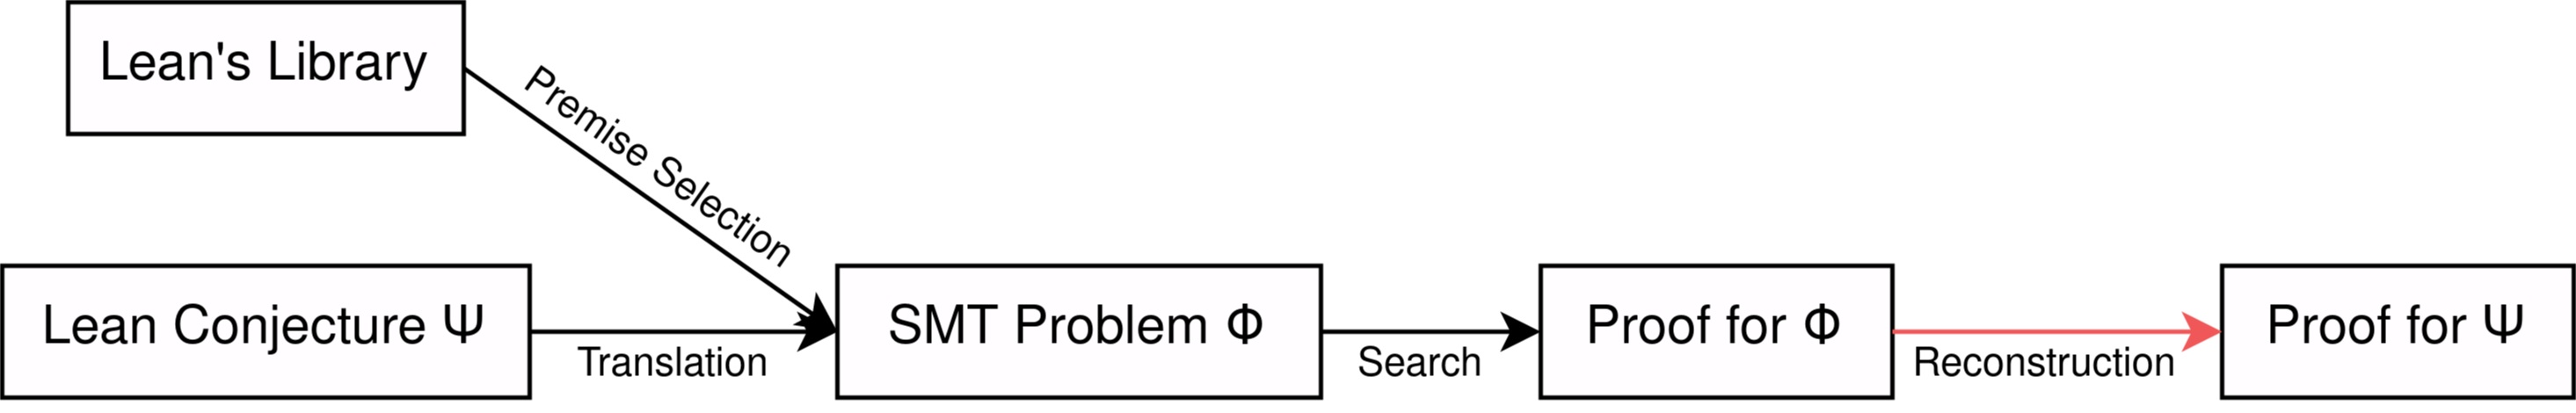
\includegraphics[height=0.26\textheight]{images/pic7.png}
% \end{frame}

\begin{frame}
  \frametitle{Another Application}
  \begin{itemize}
    \item Checking results obtained by the ATP
    \begin{itemize}
      \item Carcara is an example of other tool that does this
      \item It is much faster than our tool, but it works on a very different setting
    \end{itemize}
    \vitem The ITP is more reliable than an independent checker
    \begin{itemize}
      \item Small kernel
      \item Many users constantly testing it
    \end{itemize}
  \end{itemize}
\end{frame}



\begin{frame}
  \frametitle{Outline}
  \begin{enumerate}
    \item Introduction \bluecheck
    \vitem SMT solvers and proof certificates
    \vitem Lean
    \vitem Certified approach
    \vitem Certifying approach
    \vitem Demo
    \vitem Evaluation
  \end{enumerate}
\end{frame}

\section{SMT Solvers}

\begin{frame}
  \frametitle{The SMT Problem}
  \begin{itemize}
    \item Boolean Satisfiability Problem (SAT)
    \vitem Input: a formula with Boolean variables connected with the operators $\wedge$, $\vee$ and $\neg$
    \vitem Question: is there a way to assign values to the variables such that the formula evaluate to true?
  \end{itemize}
\end{frame}


\begin{frame}
  \frametitle{The SMT Problem}
  \begin{overprint}
    \onslide<1-2>
    \medskip
    $$\neg (x_{1} \vee x_{2}) \wedge x_{3} \wedge (\neg x_{1} \vee \neg x_{3})$$
  \end{overprint}
  \vfill
  \begin{overprint}
    \onslide<2>
    \begin{center}
      \textcolor{ForestGreen}{Satisfiable}\\
    $x_{1} \mapsto false$ \\
    $x_{2} \mapsto false$ \\
    $x_{3} \mapsto true$
    \end{center}
  \end{overprint}
\end{frame}

\begin{frame}
  \frametitle{The SMT Problem}
  \begin{overprint}
    \onslide<1-2>
    \medskip
    $$\neg (x_{1} \vee x_{2}) \wedge x_{3} \wedge (x_{1} \vee \neg x_{3})$$
  \end{overprint}
  \vfill
  \begin{overprint}
    \onslide<2>
    \begin{center}
      \color{red}Unsatisfiable
    \end{center}
  \end{overprint}
\end{frame}

\begin{frame}
  \frametitle{The SMT Problem}
  \begin{itemize}
    \item Satisfiability Modulo Theories is an extension over SAT
    \begin{itemize}
      \item We still want to check if formulas are satisfiable
    \end{itemize}
    \vitem Variables can range over different domains (sorts) apart from Boolean
    \vitem Operators from these domains are also added
  \end{itemize}
\end{frame}
\begin{frame}
  \frametitle{The SMT Problem}
  \begin{itemize}
    \item Theories we currently cover:
    \begin{itemize}
      \item Boolean (essential for capturing the reasoning over SMT formulas)
      \item Equality and Uninterpreted Functions
      \item Linear Arithmetic
    \end{itemize}
    \vitem Ongoing work:
    \begin{itemize}
      \item Non-linear arithmetic
      \item Quantifiers
    \end{itemize}
  \end{itemize}
\end{frame}


\begin{frame}
  \frametitle{The SMT Problem}
  \begin{overprint}
    \onslide<1-2>
    \medskip
    \begin{center}
      $(x > 0) \wedge (x < 2) \wedge (f(x) \not\simeq f(1))$
      % $(x_{1} > x_{2}) \wedge (x_{2} \ge 0) \wedge (x_{1} < 2) \wedge (f(x_{1}) \not\simeq f(1) \vee x_{2} > 3)$ \\
      % $ (x_{1} \ge 0) \wedge (x_{1} < 2) \wedge (x_{1} \times x_{2} \not\simeq 0) \wedge ((f(5x_{1}) \not\simeq f(5)) \vee (x_{2} \simeq 0)) $ \\

      $x \in \mathbb{Z}$ \\

      $f : \mathbb{Z} \rightarrow \mathbb{Z}$
    \end{center}
  \end{overprint}
  \vfill
  \begin{overprint}
    \onslide<2>
    \begin{center}
      \color{red}Unsatisfiable
    \end{center}
  \end{overprint}
\end{frame}

\begin{frame}
  \frametitle{SMT Solvers}
  \begin{itemize}
    \item SMT Solvers are systems that aim to solve the SMT problem
    \vitem In order to determine whether a given formula is satisfiable, they combine SAT solvers with theory specific solvers
    \vitem Most of them accept the SMT-LIB format as input
  \end{itemize}
\end{frame}

\begin{frame}[fragile]
  \frametitle{SMT Solvers}
  \begin{minted}{smtlib.py -x}
    (set-logic QF_UFLIA)

    (declare-const x Int)
    (declare-fun f (Int) Int)

    (assert (> x 0))
    (assert (< x 2))
    (assert (not (= (f x) (f 1)))

    (check-sat)
  \end{minted}
\end{frame}

\begin{frame}
  \frametitle{SMT Solvers}
  \begin{itemize}
    \item Furthermore, some SMT solvers (including cvc5) can produce a certificate that supports the result found for a given formula
    \vitem For ``SAT'' results this is easy: just show the valuation of the variables
    \vitem What about ``UNSAT'' results?
  \end{itemize}
\end{frame}

\begin{frame}
  \frametitle{Proof Certificates for Boolean Formulas}
    \begin{itemize}
    \item Initially, assume that the input formula is in Conjunctive Normal Form (CNF)
    \begin{itemize}
      \item This means that the formula is a conjunction of many clauses
      \item A clause is a disjunction of variables
    \end{itemize}
    \vitem Proof certificates for unsatisfiability of Boolean formulas in CNF rely on the \textit{resolution} rule:
          \vfill
  \[
    \infer[]{x_{1} \vee \cdots \vee x_{n} \vee y_{1} \vee \cdots \vee y_{m}}{a \vee x_{1} \vee \cdots \vee x_{n} & \neg a \vee y_{1} \vee \cdots \vee y_{m}}
  \]
  \vitem Example:
            \vfill
          $$ (x_{1} \vee \neg x_{2} \vee \neg x_{3}) \wedge (x_{4} \vee \neg x_{1}) \Rightarrow \neg x_{2} \vee \neg x_{3} \vee x_{4} $$
   \end{itemize}
\end{frame}

\begin{frame}
  \frametitle{Proof Certificates for Boolean Formulas}
  \begin{itemize}
    \item The algorithm employed by SAT solvers to solve the SAT problem relies on the resolution rule
    \vitem We can represent their reasoning with a sequence of applications of resolution
    \vitem By modifying them so they register each instance of resolution applied, we can obtain a \textit{resolution tree}, which is a suitable certificate for ``UNSAT'' result in Boolean formulas
  \end{itemize}
\end{frame}
\begin{frame}
  \frametitle{Proof Certificates for Boolean Formulas}
  \begin{itemize}
    \item Consider the formula $(x \vee y) \wedge (x \vee \neg y \vee z) \wedge (\neg x \vee z) \wedge  \neg z$. The following is a resolution tree certifying the unsatisfiability of this formula:
  \end{itemize}
  \vfill
  \[
\infer[]{\bot}{
  \infer[]
  {x}
  {x \vee y & \infer[]{x \vee \neg y}{x \vee \neg y \vee z & \neg z}} & \infer[]{\neg x}{\neg x \vee z & \neg z}}
\]
\end{frame}

\begin{frame}
  \frametitle{Proof Certificates for Boolean Formulas}
  \begin{itemize}
    \item If the input formula is \textbf{not} in CNF, the SAT solver applies a set of rules to transform it into a CNF formula
    \vitem These rules can also be captured in the same way as the resolution rule and embedded in the proof tree
  \end{itemize}
\end{frame}

\begin{frame}
  \frametitle{Proof Certificates for Boolean Formulas}
  \begin{itemize}
    \item Consider again the following unsatisfiable formula: $\neg (x_{1} \vee x_{2}) \wedge x_{3} \wedge (x_{1} \vee \neg x_{3})$
    \vitem By applying the \textit{De Morgan's Law} in the sub-expression $\neg (x_{1} \vee x_{2})$ we obtain $\neg x_{1} \wedge \neg x_{2}$
    \vitem Substituting it on the original formula, we obtain a CNF formula with 4 clauses: $\neg x_{1} \wedge \neg x_{2} \wedge x_{3} \wedge (x_{1} \vee \neg x_{3})$
  \end{itemize}

    \begin{prooftree}
      \AxiomC{$\neg (x_{1} \vee x_{2})$}
      \RightLabel{\footnotesize\textit{deMorgan}}
      \UnaryInfC{$\neg x_{1} \wedge \neg x_{2}$}
      \RightLabel{\footnotesize\textit{andElim}}
      \UnaryInfC{$\neg x_{1}$}

      \AxiomC{$x_{1} \vee \neg x_{3}$}
      \AxiomC{$x_{3}$}
      \RightLabel{\footnotesize\textit{resolution}}
      \BinaryInfC{$x_{1}$}
      \RightLabel{\footnotesize\textit{resolution}}
      \BinaryInfC{$\bot$}
    \end{prooftree}
\end{frame}

\begin{frame}
  \frametitle{Proof Certificates for Equality and Uninterpreted Functions}
  \begin{itemize}
    \item Next, we consider the theory of Equality and Uninterpreted Functions
    \vitem Formulas involving variables and functions taken from an arbitrary sort
    \vitem We also introduce an equality operator: $\simeq$
    \vitem Examples:
  \end{itemize}
  \begin{enumerate}
    \item $(b \simeq c) \wedge (f(b) \simeq c) \wedge (f(c) \simeq a) \wedge (a \not\simeq b)$
    \item $(a \simeq f(f(a))) \wedge (a \simeq f(f(f(a)))) \wedge (f(a) \not\simeq a)$
  \end{enumerate}
\end{frame}

\begin{frame}
  \frametitle{Proof Certificates for Equality and Uninterpreted Functions}
  \begin{itemize}
    \item Function applications respect the congruence property:
    \begin{itemize}
      \item If $f$ and $g$ are two functions and $x$ and $y$ are two variables, $f \simeq g$ and $x \simeq y$ imply $f(x) \simeq g(y)$
    \end{itemize}
    \vitem Proof certificates for unsatisfiability of formulas in this theory consist of proof trees in which the transitions are applications of congruence, reflexivity, symmetry and transitivity
  \end{itemize}
\end{frame}

\begin{frame}
  \frametitle{Proof Certificates for Equality and Uninterpreted Functions}
  \begin{itemize}
    \item Proof certificate for $(a \simeq f(f(a))) \wedge (a \simeq f(f(f(a)))) \wedge (f(a) \not\simeq a)$
  \end{itemize}
  \vfill
  \[
    \infer[\textit{resolution}]{\bot}{\infer[\textit{trans}]{f(a) \simeq a}{\infer[\textit{cong}]{f(a) \simeq f(f(f(a)))}{\infer[\textit{refl}]{f \simeq f}{} & a \simeq f(f(a))} & \infer[\textit{symm}]{f(f(f(a))) \simeq a}{a \simeq f(f(f(a)))}} & f(a) \not\simeq a}
  \]
\end{frame}

\begin{frame}
  \frametitle{Proof Certificates for Linear Arithmetic}
  \begin{itemize}
    \item In the theory of Linear Arithmetic, we consider variables ranging over reals or integers that can be added and scaled by constants
    \vitem General form of a term:
  \end{itemize}
  \[
    \sum_{i} a_{i} x_{i} \bowtie b
  \]
  Where $\bowtie$ is either $<$, $\le$ or $\simeq$
\end{frame}

\begin{frame}
  \frametitle{Proof Certificates for Linear Arithmetic}
  \begin{itemize}
    \item Example: $x_{1} + x_{2} \le 1 \wedge 2x_{1} - 2x_{2} \le -4 \wedge x_{1} \ge 0 \wedge x_{2} \ge 0$
    \vitem Proof certificates for unsatisfiability of formulas in LRA rely on the Farkas' lemma:
    \begin{itemize}
      \item If there is no solution for a sequence of restrictions, then there is a sequence of coefficients $s_{i}$ such that one can derive an absurd by multiplying each coefficient to the corresponding restriction and adding all scaled restrictions
    \end{itemize}
    \vitem For the example above, one can multiply the first restriction by 2 and the second by 1 and add them to obtain $4x_{1} \le -3$, which is an absurd, since another restriction says that $x_{1} \ge 0$.
  \end{itemize}
\end{frame}

\begin{frame}
  \frametitle{Proof Certificates for Linear Arithmetic}
  \begin{itemize}
    \item Since the Farkas' lemma guarantee that such coefficients always exist, the SMT solver can compute them and provide it as a proof certificate.
    % \vitem Linear Integer Arithmetic? Tight Bounds?
  \end{itemize}
\end{frame}

\begin{frame}
  \frametitle{Proof Certificates for Preprocessing Steps}
  \begin{itemize}
    \item The final proof certificate will be a combination for the formats of certificates for each theory
    \vitem The SMT solver also can perform preprocessing steps in the input formula to simplify it, which will be added in the final certificate
    \begin{itemize}
      \item An example of such simplification is rewriting known formulas, like $x + 0 = x$
    \end{itemize}
    \vitem These preprocessing steps should be justified, but cvc5 currently can't produce proof certificates for them. Instead, they are added as hypothesis in the final proof
  \end{itemize}
\end{frame}

% \begin{frame}[t]
%   \frametitle{Solver Architecture}
%   \begin{center}
%   \centering
%   \only<1>{
%     \newcommand{\preprocopacity}{0}
%     \newcommand{\nopreprocopacity}{1}
%     \newcommand{\smtopacity}{1}
%     \newcommand{\tpopacity}{0}
%     \newcommand{\detailopacityprop}{0}
%     \newcommand{\detailopacity}{0}
%     \newcommand{\proofopacity}{0}
%     \newcommand{\proofsatopacity}{0}
%     \newcommand{\proofresultopacity}{1}
%     \newcommand{\proofresultarrowopacity}{0}
%     \newcommand{\proofsmtopacity}{0}
%     \newcommand{\satopacity}{0}
%     \newcommand{\unsatopacity}{1}
%     \resizebox{0.85\linewidth}{!}{
\tikzset{every picture/.style={line width=0.75pt}}
\begin{tikzpicture}[
    block/.style={
      draw,
      minimum width=7em,
      minimum height=2em,
      fill=white,
      align=center,
    },
    theory/.style={
      draw,
      minimum width=2em,
      minimum height=2em,
      fill=white,
      align=center,
    },
  ]

  \node[opacity=\preprocopacity, block] (prep) {\textcolor{procColor}{Pre-processor}};
  \node[opacity=\nopreprocopacity] (input) {\textcolor{thRwColor}{$\varphi$}};
  \node[opacity=\preprocopacity, below=4em of prep] (phi)
    {\textcolor{thRwColor}{$\varphi$}};
  \draw[opacity=\preprocopacity, line] (phi) -- (prep);

  \node[opacity=\detailopacityprop, block, right=12ex of prep] (clause) {\textcolor{cnfColor}{Clausifier}};
  \node[opacity=\detailopacityprop, block, right=10ex of clause] (sat) {\textcolor{satColor}{SAT Solver}};
  \node[opacity=\detailopacityprop, block, right=10ex of sat] (post) {Post-processor};
  \draw[opacity=\detailopacityprop, line] (clause) -- node[above] {\scriptsize\textcolor{cnfColor}{$
    C_1^\mathrm{p}\ \ldots\ C_m^\mathrm{p}$}} (sat);
    % C_1\rrfloor_p\;...\;\llfloor C_m\rrfloor_p$} (sat);
  \draw[opacity=\proofsatopacity, line] (sat) -- node[above] {\scriptsize\textcolor{satColor}{$P\!:\vec{C}\rightarrow\bot$}} (post);
  \draw[opacity=\detailopacityprop, line] (clause.south) -- +(0,-1em) -- node[below,align=center]
  {\scriptsize\textcolor{cnfColor}{$P\!: \psi_1\rightarrow C_1\ \ldots\ P\!: \psi_m\rightarrow C_m$}} ($(post.south)+(0,-1em)$) -- (post.south);

  \node[opacity=\detailopacity, block,below=13em of clause.west,anchor=west] (comb) {\textcolor{thSolverColor}{Theory Combination}};
  \node[opacity=\detailopacity, theory,right=10ex of comb,yshift=+3em] (t1) {\textcolor{thSolverColor}{$T_1$}};
  \node[opacity=\detailopacity, theory,right=10ex of comb,yshift=-3em] (t2) {\textcolor{thSolverColor}{$T_2$}};
  \path[opacity=\detailopacity, draw,line] (t1.west) to[bend right]
    node[left,yshift=1ex]
      {\scriptsize\textcolor{thSolverColor}{$L_1\hskip .8em P\!: L_1$}}
      ($(comb.east)+(0,1ex)$);
  \path[opacity=\detailopacity, draw,line] (t2.west) to[bend left]
    node[left,yshift=-1ex]
      {\scriptsize\textcolor{thSolverColor}{$L_2\hskip .8em P\!: L_2$}}
      ($(comb.east)+(0,-1ex)$);
  \node[opacity=\detailopacity, right=6ex of comb,minimum height=4ex] (tdots) {$\ldots$};
  \node[opacity=\detailopacity, theory,right=10ex of tdots] (tk) {\textcolor{thSolverColor}{$T_k$}};
  \draw[opacity=\detailopacity, line] (tdots) -- (comb);
  \draw[opacity=\detailopacity] (tk) -- node[above]
    {\scriptsize\textcolor{thSolverColor}{$L_k\hskip .5em P\!: L_k$}} (tdots);

  \node[opacity=\proofopacity, block,right=8ex of post.east,yshift=4em] (smt) {SMT Proof Post-processor};
  \node[opacity=\proofresultopacity, below=6em of smt] (p2) {\textcolor{thRwColor}{$P\!:\varphi\rightarrow\bot$}};
  \draw[opacity=\proofresultarrowopacity, line] (smt) -- (p2);

  \node[opacity=\unsatopacity, right=10ex of post.east,yshift=-4em, anchor=center] (b2) {\textcolor{thRwColor}{$\bot$}};
  \node[opacity=\satopacity, right=10ex of post.east,yshift=4em, anchor=center] (sat) {sat};

  \path (prep.north)+(0,5em) node (p0) {};
  \draw[opacity=\proofopacity, line] (prep.north) -- +(0,5em) --
    node[above]
    {
      \textcolor{procColor}{$P\!: \varphi\rightarrow\phi_1\ \ldots\ P\!: \varphi\rightarrow\phi_n$}
    } ($(smt.north |- p0)$) -- (smt.north);

  \begin{pgfonlayer}{background}
    \path (clause.north west)+(-1.5em,7ex) node (c0) {};
    \path (post.south east)+(1.5em,-5.1ex) node (c1) {};
    \node at ($($(c1 -| c0)$)!0.5!(c1)$) (c2) {};
    \path[opacity=\tpopacity, rounded corners, draw=gray!45, fill=gray!10] (c0) rectangle (c1);

    \path (comb.west)+(-1.5em,6em) node (d0) {};
    \path (c1)+(0em,-16em) node (d1) {};
    \node at ($($(d0 -| d1)$)!0.5!(d0)$) (d2) {};
    \path[opacity=\tpopacity, rounded corners, draw=gray!45, fill=gray!10] (d0) rectangle (d1);

    \path[opacity=\smtopacity, rounded corners, draw=gray!45, fill=gray!10] (c0) rectangle (d1);
  \end{pgfonlayer}

  \node[opacity=\tpopacity, below=1ex of c0,xshift=1ex,anchor=north west] (pengine) {Propositional Engine};
  \node[opacity=\tpopacity, below=1ex of d0,xshift=1ex,anchor=north west] (tengine) {Theory Engine};
  \node[opacity=\smtopacity] at ($(c0)!0.5!(d1)$) (solver) {\textcolor{thRwColor}{SMT Solver}};

  \path[opacity=\tpopacity, draw,rline,line width=0.75pt] (d2)+(-1em,0em) to[bend left=40]
    node[left] {\textcolor{satColor}{Asserted Literals}}
    ($(c2)+(-1em,0em)$);

  \path[opacity=\detailopacity, draw,line,line width=0.75pt] (d2)+(1em,0em) to[bend right=40]
    node[right,align=center] {\textcolor{thSolverColor}{$L$}\\[.5ex]\textcolor{thSolverColor}{$P\!: L$}}
    ($(c2)+(1em,0em)$);

  \path ($(prep.east -| c0)$) node (c3) {};
  \draw[opacity=\preprocopacity, line] (prep.east) -- node[above]
    {\textcolor{procColor}{$\vec \phi$}} (c3.center);

  \draw[opacity=\nopreprocopacity, line] (input) -- (c3.center);

  \path ($(post.east -| c1)$) node (c4) {};
  \draw[opacity=\unsatopacity, line,line width=0.75pt] (c4)+(0ex,-1ex) -| (b2);

  \draw[opacity=\satopacity, line,line width=0.75pt] (c4)+(0ex,1ex) -| (sat);

  \draw[opacity=\proofsmtopacity, line,line width=0.75pt] (c4)+(0ex,1ex) -| ($(smt.south)+(-1ex,0ex)$) node[above,pos=0.25] {\textcolor{thRwColor}{$P\!:\vec \phi\rightarrow\bot$}};

\end{tikzpicture}%
}

%   }%
%   \only<2>{
%     \newcommand{\preprocopacity}{1}
%     \newcommand{\nopreprocopacity}{0}
%     \newcommand{\smtopacity}{1}
%     \newcommand{\tpopacity}{0}
%     \newcommand{\detailopacityprop}{0}
%     \newcommand{\detailopacity}{0}
%     \newcommand{\proofopacity}{0}
%     \newcommand{\proofsatopacity}{0}
%     \newcommand{\proofresultopacity}{0}
%     \newcommand{\proofresultarrowopacity}{0}
%     \newcommand{\proofsmtopacity}{0}
%     \newcommand{\satopacity}{0}
%     \newcommand{\unsatopacity}{0}
%     \resizebox{0.85\linewidth}{!}{
\tikzset{every picture/.style={line width=0.75pt}}
\begin{tikzpicture}[
    block/.style={
      draw,
      minimum width=7em,
      minimum height=2em,
      fill=white,
      align=center,
    },
    theory/.style={
      draw,
      minimum width=2em,
      minimum height=2em,
      fill=white,
      align=center,
    },
  ]

  \node[opacity=\preprocopacity, block] (prep) {\textcolor{procColor}{Pre-processor}};
  \node[opacity=\nopreprocopacity] (input) {\textcolor{thRwColor}{$\varphi$}};
  \node[opacity=\preprocopacity, below=4em of prep] (phi)
    {\textcolor{thRwColor}{$\varphi$}};
  \draw[opacity=\preprocopacity, line] (phi) -- (prep);

  \node[opacity=\detailopacityprop, block, right=12ex of prep] (clause) {\textcolor{cnfColor}{Clausifier}};
  \node[opacity=\detailopacityprop, block, right=10ex of clause] (sat) {\textcolor{satColor}{SAT Solver}};
  \node[opacity=\detailopacityprop, block, right=10ex of sat] (post) {Post-processor};
  \draw[opacity=\detailopacityprop, line] (clause) -- node[above] {\scriptsize\textcolor{cnfColor}{$
    C_1^\mathrm{p}\ \ldots\ C_m^\mathrm{p}$}} (sat);
    % C_1\rrfloor_p\;...\;\llfloor C_m\rrfloor_p$} (sat);
  \draw[opacity=\proofsatopacity, line] (sat) -- node[above] {\scriptsize\textcolor{satColor}{$P\!:\vec{C}\rightarrow\bot$}} (post);
  \draw[opacity=\detailopacityprop, line] (clause.south) -- +(0,-1em) -- node[below,align=center]
  {\scriptsize\textcolor{cnfColor}{$P\!: \psi_1\rightarrow C_1\ \ldots\ P\!: \psi_m\rightarrow C_m$}} ($(post.south)+(0,-1em)$) -- (post.south);

  \node[opacity=\detailopacity, block,below=13em of clause.west,anchor=west] (comb) {\textcolor{thSolverColor}{Theory Combination}};
  \node[opacity=\detailopacity, theory,right=10ex of comb,yshift=+3em] (t1) {\textcolor{thSolverColor}{$T_1$}};
  \node[opacity=\detailopacity, theory,right=10ex of comb,yshift=-3em] (t2) {\textcolor{thSolverColor}{$T_2$}};
  \path[opacity=\detailopacity, draw,line] (t1.west) to[bend right]
    node[left,yshift=1ex]
      {\scriptsize\textcolor{thSolverColor}{$L_1\hskip .8em P\!: L_1$}}
      ($(comb.east)+(0,1ex)$);
  \path[opacity=\detailopacity, draw,line] (t2.west) to[bend left]
    node[left,yshift=-1ex]
      {\scriptsize\textcolor{thSolverColor}{$L_2\hskip .8em P\!: L_2$}}
      ($(comb.east)+(0,-1ex)$);
  \node[opacity=\detailopacity, right=6ex of comb,minimum height=4ex] (tdots) {$\ldots$};
  \node[opacity=\detailopacity, theory,right=10ex of tdots] (tk) {\textcolor{thSolverColor}{$T_k$}};
  \draw[opacity=\detailopacity, line] (tdots) -- (comb);
  \draw[opacity=\detailopacity] (tk) -- node[above]
    {\scriptsize\textcolor{thSolverColor}{$L_k\hskip .5em P\!: L_k$}} (tdots);

  \node[opacity=\proofopacity, block,right=8ex of post.east,yshift=4em] (smt) {SMT Proof Post-processor};
  \node[opacity=\proofresultopacity, below=6em of smt] (p2) {\textcolor{thRwColor}{$P\!:\varphi\rightarrow\bot$}};
  \draw[opacity=\proofresultarrowopacity, line] (smt) -- (p2);

  \node[opacity=\unsatopacity, right=10ex of post.east,yshift=-4em, anchor=center] (b2) {\textcolor{thRwColor}{$\bot$}};
  \node[opacity=\satopacity, right=10ex of post.east,yshift=4em, anchor=center] (sat) {sat};

  \path (prep.north)+(0,5em) node (p0) {};
  \draw[opacity=\proofopacity, line] (prep.north) -- +(0,5em) --
    node[above]
    {
      \textcolor{procColor}{$P\!: \varphi\rightarrow\phi_1\ \ldots\ P\!: \varphi\rightarrow\phi_n$}
    } ($(smt.north |- p0)$) -- (smt.north);

  \begin{pgfonlayer}{background}
    \path (clause.north west)+(-1.5em,7ex) node (c0) {};
    \path (post.south east)+(1.5em,-5.1ex) node (c1) {};
    \node at ($($(c1 -| c0)$)!0.5!(c1)$) (c2) {};
    \path[opacity=\tpopacity, rounded corners, draw=gray!45, fill=gray!10] (c0) rectangle (c1);

    \path (comb.west)+(-1.5em,6em) node (d0) {};
    \path (c1)+(0em,-16em) node (d1) {};
    \node at ($($(d0 -| d1)$)!0.5!(d0)$) (d2) {};
    \path[opacity=\tpopacity, rounded corners, draw=gray!45, fill=gray!10] (d0) rectangle (d1);

    \path[opacity=\smtopacity, rounded corners, draw=gray!45, fill=gray!10] (c0) rectangle (d1);
  \end{pgfonlayer}

  \node[opacity=\tpopacity, below=1ex of c0,xshift=1ex,anchor=north west] (pengine) {Propositional Engine};
  \node[opacity=\tpopacity, below=1ex of d0,xshift=1ex,anchor=north west] (tengine) {Theory Engine};
  \node[opacity=\smtopacity] at ($(c0)!0.5!(d1)$) (solver) {\textcolor{thRwColor}{SMT Solver}};

  \path[opacity=\tpopacity, draw,rline,line width=0.75pt] (d2)+(-1em,0em) to[bend left=40]
    node[left] {\textcolor{satColor}{Asserted Literals}}
    ($(c2)+(-1em,0em)$);

  \path[opacity=\detailopacity, draw,line,line width=0.75pt] (d2)+(1em,0em) to[bend right=40]
    node[right,align=center] {\textcolor{thSolverColor}{$L$}\\[.5ex]\textcolor{thSolverColor}{$P\!: L$}}
    ($(c2)+(1em,0em)$);

  \path ($(prep.east -| c0)$) node (c3) {};
  \draw[opacity=\preprocopacity, line] (prep.east) -- node[above]
    {\textcolor{procColor}{$\vec \phi$}} (c3.center);

  \draw[opacity=\nopreprocopacity, line] (input) -- (c3.center);

  \path ($(post.east -| c1)$) node (c4) {};
  \draw[opacity=\unsatopacity, line,line width=0.75pt] (c4)+(0ex,-1ex) -| (b2);

  \draw[opacity=\satopacity, line,line width=0.75pt] (c4)+(0ex,1ex) -| (sat);

  \draw[opacity=\proofsmtopacity, line,line width=0.75pt] (c4)+(0ex,1ex) -| ($(smt.south)+(-1ex,0ex)$) node[above,pos=0.25] {\textcolor{thRwColor}{$P\!:\vec \phi\rightarrow\bot$}};

\end{tikzpicture}%
}

%   }%
%   \only<3>{
%     \newcommand{\preprocopacity}{1}
%     \newcommand{\nopreprocopacity}{0}
%     \newcommand{\smtopacity}{1}
%     \newcommand{\tpopacity}{0}
%     \newcommand{\detailopacityprop}{0}
%     \newcommand{\detailopacity}{0}
%     \newcommand{\proofopacity}{1}
%     \newcommand{\proofsatopacity}{0}
%     \newcommand{\proofresultopacity}{0}
%     \newcommand{\proofresultarrowopacity}{0}
%     \newcommand{\proofsmtopacity}{0}
%     \newcommand{\satopacity}{0}
%     \newcommand{\unsatopacity}{0}
%     \resizebox{0.85\linewidth}{!}{
\tikzset{every picture/.style={line width=0.75pt}}
\begin{tikzpicture}[
    block/.style={
      draw,
      minimum width=7em,
      minimum height=2em,
      fill=white,
      align=center,
    },
    theory/.style={
      draw,
      minimum width=2em,
      minimum height=2em,
      fill=white,
      align=center,
    },
  ]

  \node[opacity=\preprocopacity, block] (prep) {\textcolor{procColor}{Pre-processor}};
  \node[opacity=\nopreprocopacity] (input) {\textcolor{thRwColor}{$\varphi$}};
  \node[opacity=\preprocopacity, below=4em of prep] (phi)
    {\textcolor{thRwColor}{$\varphi$}};
  \draw[opacity=\preprocopacity, line] (phi) -- (prep);

  \node[opacity=\detailopacityprop, block, right=12ex of prep] (clause) {\textcolor{cnfColor}{Clausifier}};
  \node[opacity=\detailopacityprop, block, right=10ex of clause] (sat) {\textcolor{satColor}{SAT Solver}};
  \node[opacity=\detailopacityprop, block, right=10ex of sat] (post) {Post-processor};
  \draw[opacity=\detailopacityprop, line] (clause) -- node[above] {\scriptsize\textcolor{cnfColor}{$
    C_1^\mathrm{p}\ \ldots\ C_m^\mathrm{p}$}} (sat);
    % C_1\rrfloor_p\;...\;\llfloor C_m\rrfloor_p$} (sat);
  \draw[opacity=\proofsatopacity, line] (sat) -- node[above] {\scriptsize\textcolor{satColor}{$P\!:\vec{C}\rightarrow\bot$}} (post);
  \draw[opacity=\detailopacityprop, line] (clause.south) -- +(0,-1em) -- node[below,align=center]
  {\scriptsize\textcolor{cnfColor}{$P\!: \psi_1\rightarrow C_1\ \ldots\ P\!: \psi_m\rightarrow C_m$}} ($(post.south)+(0,-1em)$) -- (post.south);

  \node[opacity=\detailopacity, block,below=13em of clause.west,anchor=west] (comb) {\textcolor{thSolverColor}{Theory Combination}};
  \node[opacity=\detailopacity, theory,right=10ex of comb,yshift=+3em] (t1) {\textcolor{thSolverColor}{$T_1$}};
  \node[opacity=\detailopacity, theory,right=10ex of comb,yshift=-3em] (t2) {\textcolor{thSolverColor}{$T_2$}};
  \path[opacity=\detailopacity, draw,line] (t1.west) to[bend right]
    node[left,yshift=1ex]
      {\scriptsize\textcolor{thSolverColor}{$L_1\hskip .8em P\!: L_1$}}
      ($(comb.east)+(0,1ex)$);
  \path[opacity=\detailopacity, draw,line] (t2.west) to[bend left]
    node[left,yshift=-1ex]
      {\scriptsize\textcolor{thSolverColor}{$L_2\hskip .8em P\!: L_2$}}
      ($(comb.east)+(0,-1ex)$);
  \node[opacity=\detailopacity, right=6ex of comb,minimum height=4ex] (tdots) {$\ldots$};
  \node[opacity=\detailopacity, theory,right=10ex of tdots] (tk) {\textcolor{thSolverColor}{$T_k$}};
  \draw[opacity=\detailopacity, line] (tdots) -- (comb);
  \draw[opacity=\detailopacity] (tk) -- node[above]
    {\scriptsize\textcolor{thSolverColor}{$L_k\hskip .5em P\!: L_k$}} (tdots);

  \node[opacity=\proofopacity, block,right=8ex of post.east,yshift=4em] (smt) {SMT Proof Post-processor};
  \node[opacity=\proofresultopacity, below=6em of smt] (p2) {\textcolor{thRwColor}{$P\!:\varphi\rightarrow\bot$}};
  \draw[opacity=\proofresultarrowopacity, line] (smt) -- (p2);

  \node[opacity=\unsatopacity, right=10ex of post.east,yshift=-4em, anchor=center] (b2) {\textcolor{thRwColor}{$\bot$}};
  \node[opacity=\satopacity, right=10ex of post.east,yshift=4em, anchor=center] (sat) {sat};

  \path (prep.north)+(0,5em) node (p0) {};
  \draw[opacity=\proofopacity, line] (prep.north) -- +(0,5em) --
    node[above]
    {
      \textcolor{procColor}{$P\!: \varphi\rightarrow\phi_1\ \ldots\ P\!: \varphi\rightarrow\phi_n$}
    } ($(smt.north |- p0)$) -- (smt.north);

  \begin{pgfonlayer}{background}
    \path (clause.north west)+(-1.5em,7ex) node (c0) {};
    \path (post.south east)+(1.5em,-5.1ex) node (c1) {};
    \node at ($($(c1 -| c0)$)!0.5!(c1)$) (c2) {};
    \path[opacity=\tpopacity, rounded corners, draw=gray!45, fill=gray!10] (c0) rectangle (c1);

    \path (comb.west)+(-1.5em,6em) node (d0) {};
    \path (c1)+(0em,-16em) node (d1) {};
    \node at ($($(d0 -| d1)$)!0.5!(d0)$) (d2) {};
    \path[opacity=\tpopacity, rounded corners, draw=gray!45, fill=gray!10] (d0) rectangle (d1);

    \path[opacity=\smtopacity, rounded corners, draw=gray!45, fill=gray!10] (c0) rectangle (d1);
  \end{pgfonlayer}

  \node[opacity=\tpopacity, below=1ex of c0,xshift=1ex,anchor=north west] (pengine) {Propositional Engine};
  \node[opacity=\tpopacity, below=1ex of d0,xshift=1ex,anchor=north west] (tengine) {Theory Engine};
  \node[opacity=\smtopacity] at ($(c0)!0.5!(d1)$) (solver) {\textcolor{thRwColor}{SMT Solver}};

  \path[opacity=\tpopacity, draw,rline,line width=0.75pt] (d2)+(-1em,0em) to[bend left=40]
    node[left] {\textcolor{satColor}{Asserted Literals}}
    ($(c2)+(-1em,0em)$);

  \path[opacity=\detailopacity, draw,line,line width=0.75pt] (d2)+(1em,0em) to[bend right=40]
    node[right,align=center] {\textcolor{thSolverColor}{$L$}\\[.5ex]\textcolor{thSolverColor}{$P\!: L$}}
    ($(c2)+(1em,0em)$);

  \path ($(prep.east -| c0)$) node (c3) {};
  \draw[opacity=\preprocopacity, line] (prep.east) -- node[above]
    {\textcolor{procColor}{$\vec \phi$}} (c3.center);

  \draw[opacity=\nopreprocopacity, line] (input) -- (c3.center);

  \path ($(post.east -| c1)$) node (c4) {};
  \draw[opacity=\unsatopacity, line,line width=0.75pt] (c4)+(0ex,-1ex) -| (b2);

  \draw[opacity=\satopacity, line,line width=0.75pt] (c4)+(0ex,1ex) -| (sat);

  \draw[opacity=\proofsmtopacity, line,line width=0.75pt] (c4)+(0ex,1ex) -| ($(smt.south)+(-1ex,0ex)$) node[above,pos=0.25] {\textcolor{thRwColor}{$P\!:\vec \phi\rightarrow\bot$}};

\end{tikzpicture}%
}

%   }%
%   \only<4>{
%     \newcommand{\preprocopacity}{1}
%     \newcommand{\nopreprocopacity}{0}
%     \newcommand{\smtopacity}{0}
%     \newcommand{\tpopacity}{1}
%     \newcommand{\detailopacityprop}{1}
%     \newcommand{\detailopacity}{0}
%     \newcommand{\proofopacity}{1}
%     \newcommand{\proofsatopacity}{0}
%     \newcommand{\proofresultopacity}{0}
%     \newcommand{\proofresultarrowopacity}{0}
%     \newcommand{\proofsmtopacity}{0}
%     \newcommand{\satopacity}{0}
%     \newcommand{\unsatopacity}{0}
%     \resizebox{0.85\linewidth}{!}{
\tikzset{every picture/.style={line width=0.75pt}}
\begin{tikzpicture}[
    block/.style={
      draw,
      minimum width=7em,
      minimum height=2em,
      fill=white,
      align=center,
    },
    theory/.style={
      draw,
      minimum width=2em,
      minimum height=2em,
      fill=white,
      align=center,
    },
  ]

  \node[opacity=\preprocopacity, block] (prep) {\textcolor{procColor}{Pre-processor}};
  \node[opacity=\nopreprocopacity] (input) {\textcolor{thRwColor}{$\varphi$}};
  \node[opacity=\preprocopacity, below=4em of prep] (phi)
    {\textcolor{thRwColor}{$\varphi$}};
  \draw[opacity=\preprocopacity, line] (phi) -- (prep);

  \node[opacity=\detailopacityprop, block, right=12ex of prep] (clause) {\textcolor{cnfColor}{Clausifier}};
  \node[opacity=\detailopacityprop, block, right=10ex of clause] (sat) {\textcolor{satColor}{SAT Solver}};
  \node[opacity=\detailopacityprop, block, right=10ex of sat] (post) {Post-processor};
  \draw[opacity=\detailopacityprop, line] (clause) -- node[above] {\scriptsize\textcolor{cnfColor}{$
    C_1^\mathrm{p}\ \ldots\ C_m^\mathrm{p}$}} (sat);
    % C_1\rrfloor_p\;...\;\llfloor C_m\rrfloor_p$} (sat);
  \draw[opacity=\proofsatopacity, line] (sat) -- node[above] {\scriptsize\textcolor{satColor}{$P\!:\vec{C}\rightarrow\bot$}} (post);
  \draw[opacity=\detailopacityprop, line] (clause.south) -- +(0,-1em) -- node[below,align=center]
  {\scriptsize\textcolor{cnfColor}{$P\!: \psi_1\rightarrow C_1\ \ldots\ P\!: \psi_m\rightarrow C_m$}} ($(post.south)+(0,-1em)$) -- (post.south);

  \node[opacity=\detailopacity, block,below=13em of clause.west,anchor=west] (comb) {\textcolor{thSolverColor}{Theory Combination}};
  \node[opacity=\detailopacity, theory,right=10ex of comb,yshift=+3em] (t1) {\textcolor{thSolverColor}{$T_1$}};
  \node[opacity=\detailopacity, theory,right=10ex of comb,yshift=-3em] (t2) {\textcolor{thSolverColor}{$T_2$}};
  \path[opacity=\detailopacity, draw,line] (t1.west) to[bend right]
    node[left,yshift=1ex]
      {\scriptsize\textcolor{thSolverColor}{$L_1\hskip .8em P\!: L_1$}}
      ($(comb.east)+(0,1ex)$);
  \path[opacity=\detailopacity, draw,line] (t2.west) to[bend left]
    node[left,yshift=-1ex]
      {\scriptsize\textcolor{thSolverColor}{$L_2\hskip .8em P\!: L_2$}}
      ($(comb.east)+(0,-1ex)$);
  \node[opacity=\detailopacity, right=6ex of comb,minimum height=4ex] (tdots) {$\ldots$};
  \node[opacity=\detailopacity, theory,right=10ex of tdots] (tk) {\textcolor{thSolverColor}{$T_k$}};
  \draw[opacity=\detailopacity, line] (tdots) -- (comb);
  \draw[opacity=\detailopacity] (tk) -- node[above]
    {\scriptsize\textcolor{thSolverColor}{$L_k\hskip .5em P\!: L_k$}} (tdots);

  \node[opacity=\proofopacity, block,right=8ex of post.east,yshift=4em] (smt) {SMT Proof Post-processor};
  \node[opacity=\proofresultopacity, below=6em of smt] (p2) {\textcolor{thRwColor}{$P\!:\varphi\rightarrow\bot$}};
  \draw[opacity=\proofresultarrowopacity, line] (smt) -- (p2);

  \node[opacity=\unsatopacity, right=10ex of post.east,yshift=-4em, anchor=center] (b2) {\textcolor{thRwColor}{$\bot$}};
  \node[opacity=\satopacity, right=10ex of post.east,yshift=4em, anchor=center] (sat) {sat};

  \path (prep.north)+(0,5em) node (p0) {};
  \draw[opacity=\proofopacity, line] (prep.north) -- +(0,5em) --
    node[above]
    {
      \textcolor{procColor}{$P\!: \varphi\rightarrow\phi_1\ \ldots\ P\!: \varphi\rightarrow\phi_n$}
    } ($(smt.north |- p0)$) -- (smt.north);

  \begin{pgfonlayer}{background}
    \path (clause.north west)+(-1.5em,7ex) node (c0) {};
    \path (post.south east)+(1.5em,-5.1ex) node (c1) {};
    \node at ($($(c1 -| c0)$)!0.5!(c1)$) (c2) {};
    \path[opacity=\tpopacity, rounded corners, draw=gray!45, fill=gray!10] (c0) rectangle (c1);

    \path (comb.west)+(-1.5em,6em) node (d0) {};
    \path (c1)+(0em,-16em) node (d1) {};
    \node at ($($(d0 -| d1)$)!0.5!(d0)$) (d2) {};
    \path[opacity=\tpopacity, rounded corners, draw=gray!45, fill=gray!10] (d0) rectangle (d1);

    \path[opacity=\smtopacity, rounded corners, draw=gray!45, fill=gray!10] (c0) rectangle (d1);
  \end{pgfonlayer}

  \node[opacity=\tpopacity, below=1ex of c0,xshift=1ex,anchor=north west] (pengine) {Propositional Engine};
  \node[opacity=\tpopacity, below=1ex of d0,xshift=1ex,anchor=north west] (tengine) {Theory Engine};
  \node[opacity=\smtopacity] at ($(c0)!0.5!(d1)$) (solver) {\textcolor{thRwColor}{SMT Solver}};

  \path[opacity=\tpopacity, draw,rline,line width=0.75pt] (d2)+(-1em,0em) to[bend left=40]
    node[left] {\textcolor{satColor}{Asserted Literals}}
    ($(c2)+(-1em,0em)$);

  \path[opacity=\detailopacity, draw,line,line width=0.75pt] (d2)+(1em,0em) to[bend right=40]
    node[right,align=center] {\textcolor{thSolverColor}{$L$}\\[.5ex]\textcolor{thSolverColor}{$P\!: L$}}
    ($(c2)+(1em,0em)$);

  \path ($(prep.east -| c0)$) node (c3) {};
  \draw[opacity=\preprocopacity, line] (prep.east) -- node[above]
    {\textcolor{procColor}{$\vec \phi$}} (c3.center);

  \draw[opacity=\nopreprocopacity, line] (input) -- (c3.center);

  \path ($(post.east -| c1)$) node (c4) {};
  \draw[opacity=\unsatopacity, line,line width=0.75pt] (c4)+(0ex,-1ex) -| (b2);

  \draw[opacity=\satopacity, line,line width=0.75pt] (c4)+(0ex,1ex) -| (sat);

  \draw[opacity=\proofsmtopacity, line,line width=0.75pt] (c4)+(0ex,1ex) -| ($(smt.south)+(-1ex,0ex)$) node[above,pos=0.25] {\textcolor{thRwColor}{$P\!:\vec \phi\rightarrow\bot$}};

\end{tikzpicture}%
}

%   }%
%   \only<5>{
%     \newcommand{\preprocopacity}{1}
%     \newcommand{\nopreprocopacity}{0}
%     \newcommand{\smtopacity}{0}
%     \newcommand{\tpopacity}{1}
%     \newcommand{\detailopacityprop}{1}
%     \newcommand{\detailopacity}{1}
%     \newcommand{\proofopacity}{1}
%     \newcommand{\proofsatopacity}{0}
%     \newcommand{\proofresultopacity}{0}
%     \newcommand{\proofresultarrowopacity}{0}
%     \newcommand{\proofsmtopacity}{0}
%     \newcommand{\satopacity}{0}
%     \newcommand{\unsatopacity}{0}
%     \resizebox{0.85\linewidth}{!}{
\tikzset{every picture/.style={line width=0.75pt}}
\begin{tikzpicture}[
    block/.style={
      draw,
      minimum width=7em,
      minimum height=2em,
      fill=white,
      align=center,
    },
    theory/.style={
      draw,
      minimum width=2em,
      minimum height=2em,
      fill=white,
      align=center,
    },
  ]

  \node[opacity=\preprocopacity, block] (prep) {\textcolor{procColor}{Pre-processor}};
  \node[opacity=\nopreprocopacity] (input) {\textcolor{thRwColor}{$\varphi$}};
  \node[opacity=\preprocopacity, below=4em of prep] (phi)
    {\textcolor{thRwColor}{$\varphi$}};
  \draw[opacity=\preprocopacity, line] (phi) -- (prep);

  \node[opacity=\detailopacityprop, block, right=12ex of prep] (clause) {\textcolor{cnfColor}{Clausifier}};
  \node[opacity=\detailopacityprop, block, right=10ex of clause] (sat) {\textcolor{satColor}{SAT Solver}};
  \node[opacity=\detailopacityprop, block, right=10ex of sat] (post) {Post-processor};
  \draw[opacity=\detailopacityprop, line] (clause) -- node[above] {\scriptsize\textcolor{cnfColor}{$
    C_1^\mathrm{p}\ \ldots\ C_m^\mathrm{p}$}} (sat);
    % C_1\rrfloor_p\;...\;\llfloor C_m\rrfloor_p$} (sat);
  \draw[opacity=\proofsatopacity, line] (sat) -- node[above] {\scriptsize\textcolor{satColor}{$P\!:\vec{C}\rightarrow\bot$}} (post);
  \draw[opacity=\detailopacityprop, line] (clause.south) -- +(0,-1em) -- node[below,align=center]
  {\scriptsize\textcolor{cnfColor}{$P\!: \psi_1\rightarrow C_1\ \ldots\ P\!: \psi_m\rightarrow C_m$}} ($(post.south)+(0,-1em)$) -- (post.south);

  \node[opacity=\detailopacity, block,below=13em of clause.west,anchor=west] (comb) {\textcolor{thSolverColor}{Theory Combination}};
  \node[opacity=\detailopacity, theory,right=10ex of comb,yshift=+3em] (t1) {\textcolor{thSolverColor}{$T_1$}};
  \node[opacity=\detailopacity, theory,right=10ex of comb,yshift=-3em] (t2) {\textcolor{thSolverColor}{$T_2$}};
  \path[opacity=\detailopacity, draw,line] (t1.west) to[bend right]
    node[left,yshift=1ex]
      {\scriptsize\textcolor{thSolverColor}{$L_1\hskip .8em P\!: L_1$}}
      ($(comb.east)+(0,1ex)$);
  \path[opacity=\detailopacity, draw,line] (t2.west) to[bend left]
    node[left,yshift=-1ex]
      {\scriptsize\textcolor{thSolverColor}{$L_2\hskip .8em P\!: L_2$}}
      ($(comb.east)+(0,-1ex)$);
  \node[opacity=\detailopacity, right=6ex of comb,minimum height=4ex] (tdots) {$\ldots$};
  \node[opacity=\detailopacity, theory,right=10ex of tdots] (tk) {\textcolor{thSolverColor}{$T_k$}};
  \draw[opacity=\detailopacity, line] (tdots) -- (comb);
  \draw[opacity=\detailopacity] (tk) -- node[above]
    {\scriptsize\textcolor{thSolverColor}{$L_k\hskip .5em P\!: L_k$}} (tdots);

  \node[opacity=\proofopacity, block,right=8ex of post.east,yshift=4em] (smt) {SMT Proof Post-processor};
  \node[opacity=\proofresultopacity, below=6em of smt] (p2) {\textcolor{thRwColor}{$P\!:\varphi\rightarrow\bot$}};
  \draw[opacity=\proofresultarrowopacity, line] (smt) -- (p2);

  \node[opacity=\unsatopacity, right=10ex of post.east,yshift=-4em, anchor=center] (b2) {\textcolor{thRwColor}{$\bot$}};
  \node[opacity=\satopacity, right=10ex of post.east,yshift=4em, anchor=center] (sat) {sat};

  \path (prep.north)+(0,5em) node (p0) {};
  \draw[opacity=\proofopacity, line] (prep.north) -- +(0,5em) --
    node[above]
    {
      \textcolor{procColor}{$P\!: \varphi\rightarrow\phi_1\ \ldots\ P\!: \varphi\rightarrow\phi_n$}
    } ($(smt.north |- p0)$) -- (smt.north);

  \begin{pgfonlayer}{background}
    \path (clause.north west)+(-1.5em,7ex) node (c0) {};
    \path (post.south east)+(1.5em,-5.1ex) node (c1) {};
    \node at ($($(c1 -| c0)$)!0.5!(c1)$) (c2) {};
    \path[opacity=\tpopacity, rounded corners, draw=gray!45, fill=gray!10] (c0) rectangle (c1);

    \path (comb.west)+(-1.5em,6em) node (d0) {};
    \path (c1)+(0em,-16em) node (d1) {};
    \node at ($($(d0 -| d1)$)!0.5!(d0)$) (d2) {};
    \path[opacity=\tpopacity, rounded corners, draw=gray!45, fill=gray!10] (d0) rectangle (d1);

    \path[opacity=\smtopacity, rounded corners, draw=gray!45, fill=gray!10] (c0) rectangle (d1);
  \end{pgfonlayer}

  \node[opacity=\tpopacity, below=1ex of c0,xshift=1ex,anchor=north west] (pengine) {Propositional Engine};
  \node[opacity=\tpopacity, below=1ex of d0,xshift=1ex,anchor=north west] (tengine) {Theory Engine};
  \node[opacity=\smtopacity] at ($(c0)!0.5!(d1)$) (solver) {\textcolor{thRwColor}{SMT Solver}};

  \path[opacity=\tpopacity, draw,rline,line width=0.75pt] (d2)+(-1em,0em) to[bend left=40]
    node[left] {\textcolor{satColor}{Asserted Literals}}
    ($(c2)+(-1em,0em)$);

  \path[opacity=\detailopacity, draw,line,line width=0.75pt] (d2)+(1em,0em) to[bend right=40]
    node[right,align=center] {\textcolor{thSolverColor}{$L$}\\[.5ex]\textcolor{thSolverColor}{$P\!: L$}}
    ($(c2)+(1em,0em)$);

  \path ($(prep.east -| c0)$) node (c3) {};
  \draw[opacity=\preprocopacity, line] (prep.east) -- node[above]
    {\textcolor{procColor}{$\vec \phi$}} (c3.center);

  \draw[opacity=\nopreprocopacity, line] (input) -- (c3.center);

  \path ($(post.east -| c1)$) node (c4) {};
  \draw[opacity=\unsatopacity, line,line width=0.75pt] (c4)+(0ex,-1ex) -| (b2);

  \draw[opacity=\satopacity, line,line width=0.75pt] (c4)+(0ex,1ex) -| (sat);

  \draw[opacity=\proofsmtopacity, line,line width=0.75pt] (c4)+(0ex,1ex) -| ($(smt.south)+(-1ex,0ex)$) node[above,pos=0.25] {\textcolor{thRwColor}{$P\!:\vec \phi\rightarrow\bot$}};

\end{tikzpicture}%
}

%   }%
%   \only<6>{
%     \newcommand{\preprocopacity}{1}
%     \newcommand{\nopreprocopacity}{0}
%     \newcommand{\smtopacity}{0}
%     \newcommand{\tpopacity}{1}
%     \newcommand{\detailopacityprop}{1}
%     \newcommand{\detailopacity}{1}
%     \newcommand{\proofopacity}{1}
%     \newcommand{\proofsatopacity}{1}
%     \newcommand{\proofresultopacity}{0}
%     \newcommand{\proofresultarrowopacity}{0}
%     \newcommand{\proofsmtopacity}{0}
%     \newcommand{\satopacity}{0}
%     \newcommand{\unsatopacity}{0}
%     \resizebox{0.85\linewidth}{!}{
\tikzset{every picture/.style={line width=0.75pt}}
\begin{tikzpicture}[
    block/.style={
      draw,
      minimum width=7em,
      minimum height=2em,
      fill=white,
      align=center,
    },
    theory/.style={
      draw,
      minimum width=2em,
      minimum height=2em,
      fill=white,
      align=center,
    },
  ]

  \node[opacity=\preprocopacity, block] (prep) {\textcolor{procColor}{Pre-processor}};
  \node[opacity=\nopreprocopacity] (input) {\textcolor{thRwColor}{$\varphi$}};
  \node[opacity=\preprocopacity, below=4em of prep] (phi)
    {\textcolor{thRwColor}{$\varphi$}};
  \draw[opacity=\preprocopacity, line] (phi) -- (prep);

  \node[opacity=\detailopacityprop, block, right=12ex of prep] (clause) {\textcolor{cnfColor}{Clausifier}};
  \node[opacity=\detailopacityprop, block, right=10ex of clause] (sat) {\textcolor{satColor}{SAT Solver}};
  \node[opacity=\detailopacityprop, block, right=10ex of sat] (post) {Post-processor};
  \draw[opacity=\detailopacityprop, line] (clause) -- node[above] {\scriptsize\textcolor{cnfColor}{$
    C_1^\mathrm{p}\ \ldots\ C_m^\mathrm{p}$}} (sat);
    % C_1\rrfloor_p\;...\;\llfloor C_m\rrfloor_p$} (sat);
  \draw[opacity=\proofsatopacity, line] (sat) -- node[above] {\scriptsize\textcolor{satColor}{$P\!:\vec{C}\rightarrow\bot$}} (post);
  \draw[opacity=\detailopacityprop, line] (clause.south) -- +(0,-1em) -- node[below,align=center]
  {\scriptsize\textcolor{cnfColor}{$P\!: \psi_1\rightarrow C_1\ \ldots\ P\!: \psi_m\rightarrow C_m$}} ($(post.south)+(0,-1em)$) -- (post.south);

  \node[opacity=\detailopacity, block,below=13em of clause.west,anchor=west] (comb) {\textcolor{thSolverColor}{Theory Combination}};
  \node[opacity=\detailopacity, theory,right=10ex of comb,yshift=+3em] (t1) {\textcolor{thSolverColor}{$T_1$}};
  \node[opacity=\detailopacity, theory,right=10ex of comb,yshift=-3em] (t2) {\textcolor{thSolverColor}{$T_2$}};
  \path[opacity=\detailopacity, draw,line] (t1.west) to[bend right]
    node[left,yshift=1ex]
      {\scriptsize\textcolor{thSolverColor}{$L_1\hskip .8em P\!: L_1$}}
      ($(comb.east)+(0,1ex)$);
  \path[opacity=\detailopacity, draw,line] (t2.west) to[bend left]
    node[left,yshift=-1ex]
      {\scriptsize\textcolor{thSolverColor}{$L_2\hskip .8em P\!: L_2$}}
      ($(comb.east)+(0,-1ex)$);
  \node[opacity=\detailopacity, right=6ex of comb,minimum height=4ex] (tdots) {$\ldots$};
  \node[opacity=\detailopacity, theory,right=10ex of tdots] (tk) {\textcolor{thSolverColor}{$T_k$}};
  \draw[opacity=\detailopacity, line] (tdots) -- (comb);
  \draw[opacity=\detailopacity] (tk) -- node[above]
    {\scriptsize\textcolor{thSolverColor}{$L_k\hskip .5em P\!: L_k$}} (tdots);

  \node[opacity=\proofopacity, block,right=8ex of post.east,yshift=4em] (smt) {SMT Proof Post-processor};
  \node[opacity=\proofresultopacity, below=6em of smt] (p2) {\textcolor{thRwColor}{$P\!:\varphi\rightarrow\bot$}};
  \draw[opacity=\proofresultarrowopacity, line] (smt) -- (p2);

  \node[opacity=\unsatopacity, right=10ex of post.east,yshift=-4em, anchor=center] (b2) {\textcolor{thRwColor}{$\bot$}};
  \node[opacity=\satopacity, right=10ex of post.east,yshift=4em, anchor=center] (sat) {sat};

  \path (prep.north)+(0,5em) node (p0) {};
  \draw[opacity=\proofopacity, line] (prep.north) -- +(0,5em) --
    node[above]
    {
      \textcolor{procColor}{$P\!: \varphi\rightarrow\phi_1\ \ldots\ P\!: \varphi\rightarrow\phi_n$}
    } ($(smt.north |- p0)$) -- (smt.north);

  \begin{pgfonlayer}{background}
    \path (clause.north west)+(-1.5em,7ex) node (c0) {};
    \path (post.south east)+(1.5em,-5.1ex) node (c1) {};
    \node at ($($(c1 -| c0)$)!0.5!(c1)$) (c2) {};
    \path[opacity=\tpopacity, rounded corners, draw=gray!45, fill=gray!10] (c0) rectangle (c1);

    \path (comb.west)+(-1.5em,6em) node (d0) {};
    \path (c1)+(0em,-16em) node (d1) {};
    \node at ($($(d0 -| d1)$)!0.5!(d0)$) (d2) {};
    \path[opacity=\tpopacity, rounded corners, draw=gray!45, fill=gray!10] (d0) rectangle (d1);

    \path[opacity=\smtopacity, rounded corners, draw=gray!45, fill=gray!10] (c0) rectangle (d1);
  \end{pgfonlayer}

  \node[opacity=\tpopacity, below=1ex of c0,xshift=1ex,anchor=north west] (pengine) {Propositional Engine};
  \node[opacity=\tpopacity, below=1ex of d0,xshift=1ex,anchor=north west] (tengine) {Theory Engine};
  \node[opacity=\smtopacity] at ($(c0)!0.5!(d1)$) (solver) {\textcolor{thRwColor}{SMT Solver}};

  \path[opacity=\tpopacity, draw,rline,line width=0.75pt] (d2)+(-1em,0em) to[bend left=40]
    node[left] {\textcolor{satColor}{Asserted Literals}}
    ($(c2)+(-1em,0em)$);

  \path[opacity=\detailopacity, draw,line,line width=0.75pt] (d2)+(1em,0em) to[bend right=40]
    node[right,align=center] {\textcolor{thSolverColor}{$L$}\\[.5ex]\textcolor{thSolverColor}{$P\!: L$}}
    ($(c2)+(1em,0em)$);

  \path ($(prep.east -| c0)$) node (c3) {};
  \draw[opacity=\preprocopacity, line] (prep.east) -- node[above]
    {\textcolor{procColor}{$\vec \phi$}} (c3.center);

  \draw[opacity=\nopreprocopacity, line] (input) -- (c3.center);

  \path ($(post.east -| c1)$) node (c4) {};
  \draw[opacity=\unsatopacity, line,line width=0.75pt] (c4)+(0ex,-1ex) -| (b2);

  \draw[opacity=\satopacity, line,line width=0.75pt] (c4)+(0ex,1ex) -| (sat);

  \draw[opacity=\proofsmtopacity, line,line width=0.75pt] (c4)+(0ex,1ex) -| ($(smt.south)+(-1ex,0ex)$) node[above,pos=0.25] {\textcolor{thRwColor}{$P\!:\vec \phi\rightarrow\bot$}};

\end{tikzpicture}%
}

%   }%
%   \only<7>{
%     \newcommand{\preprocopacity}{1}
%     \newcommand{\nopreprocopacity}{0}
%     \newcommand{\smtopacity}{0}
%     \newcommand{\tpopacity}{1}
%     \newcommand{\detailopacityprop}{1}
%     \newcommand{\detailopacity}{1}
%     \newcommand{\proofopacity}{1}
%     \newcommand{\proofsatopacity}{1}
%     \newcommand{\proofresultopacity}{0}
%     \newcommand{\proofresultarrowopacity}{0}
%     \newcommand{\proofsmtopacity}{1}
%     \newcommand{\satopacity}{0}
%     \newcommand{\unsatopacity}{1}
%     \resizebox{0.85\linewidth}{!}{
\tikzset{every picture/.style={line width=0.75pt}}
\begin{tikzpicture}[
    block/.style={
      draw,
      minimum width=7em,
      minimum height=2em,
      fill=white,
      align=center,
    },
    theory/.style={
      draw,
      minimum width=2em,
      minimum height=2em,
      fill=white,
      align=center,
    },
  ]

  \node[opacity=\preprocopacity, block] (prep) {\textcolor{procColor}{Pre-processor}};
  \node[opacity=\nopreprocopacity] (input) {\textcolor{thRwColor}{$\varphi$}};
  \node[opacity=\preprocopacity, below=4em of prep] (phi)
    {\textcolor{thRwColor}{$\varphi$}};
  \draw[opacity=\preprocopacity, line] (phi) -- (prep);

  \node[opacity=\detailopacityprop, block, right=12ex of prep] (clause) {\textcolor{cnfColor}{Clausifier}};
  \node[opacity=\detailopacityprop, block, right=10ex of clause] (sat) {\textcolor{satColor}{SAT Solver}};
  \node[opacity=\detailopacityprop, block, right=10ex of sat] (post) {Post-processor};
  \draw[opacity=\detailopacityprop, line] (clause) -- node[above] {\scriptsize\textcolor{cnfColor}{$
    C_1^\mathrm{p}\ \ldots\ C_m^\mathrm{p}$}} (sat);
    % C_1\rrfloor_p\;...\;\llfloor C_m\rrfloor_p$} (sat);
  \draw[opacity=\proofsatopacity, line] (sat) -- node[above] {\scriptsize\textcolor{satColor}{$P\!:\vec{C}\rightarrow\bot$}} (post);
  \draw[opacity=\detailopacityprop, line] (clause.south) -- +(0,-1em) -- node[below,align=center]
  {\scriptsize\textcolor{cnfColor}{$P\!: \psi_1\rightarrow C_1\ \ldots\ P\!: \psi_m\rightarrow C_m$}} ($(post.south)+(0,-1em)$) -- (post.south);

  \node[opacity=\detailopacity, block,below=13em of clause.west,anchor=west] (comb) {\textcolor{thSolverColor}{Theory Combination}};
  \node[opacity=\detailopacity, theory,right=10ex of comb,yshift=+3em] (t1) {\textcolor{thSolverColor}{$T_1$}};
  \node[opacity=\detailopacity, theory,right=10ex of comb,yshift=-3em] (t2) {\textcolor{thSolverColor}{$T_2$}};
  \path[opacity=\detailopacity, draw,line] (t1.west) to[bend right]
    node[left,yshift=1ex]
      {\scriptsize\textcolor{thSolverColor}{$L_1\hskip .8em P\!: L_1$}}
      ($(comb.east)+(0,1ex)$);
  \path[opacity=\detailopacity, draw,line] (t2.west) to[bend left]
    node[left,yshift=-1ex]
      {\scriptsize\textcolor{thSolverColor}{$L_2\hskip .8em P\!: L_2$}}
      ($(comb.east)+(0,-1ex)$);
  \node[opacity=\detailopacity, right=6ex of comb,minimum height=4ex] (tdots) {$\ldots$};
  \node[opacity=\detailopacity, theory,right=10ex of tdots] (tk) {\textcolor{thSolverColor}{$T_k$}};
  \draw[opacity=\detailopacity, line] (tdots) -- (comb);
  \draw[opacity=\detailopacity] (tk) -- node[above]
    {\scriptsize\textcolor{thSolverColor}{$L_k\hskip .5em P\!: L_k$}} (tdots);

  \node[opacity=\proofopacity, block,right=8ex of post.east,yshift=4em] (smt) {SMT Proof Post-processor};
  \node[opacity=\proofresultopacity, below=6em of smt] (p2) {\textcolor{thRwColor}{$P\!:\varphi\rightarrow\bot$}};
  \draw[opacity=\proofresultarrowopacity, line] (smt) -- (p2);

  \node[opacity=\unsatopacity, right=10ex of post.east,yshift=-4em, anchor=center] (b2) {\textcolor{thRwColor}{$\bot$}};
  \node[opacity=\satopacity, right=10ex of post.east,yshift=4em, anchor=center] (sat) {sat};

  \path (prep.north)+(0,5em) node (p0) {};
  \draw[opacity=\proofopacity, line] (prep.north) -- +(0,5em) --
    node[above]
    {
      \textcolor{procColor}{$P\!: \varphi\rightarrow\phi_1\ \ldots\ P\!: \varphi\rightarrow\phi_n$}
    } ($(smt.north |- p0)$) -- (smt.north);

  \begin{pgfonlayer}{background}
    \path (clause.north west)+(-1.5em,7ex) node (c0) {};
    \path (post.south east)+(1.5em,-5.1ex) node (c1) {};
    \node at ($($(c1 -| c0)$)!0.5!(c1)$) (c2) {};
    \path[opacity=\tpopacity, rounded corners, draw=gray!45, fill=gray!10] (c0) rectangle (c1);

    \path (comb.west)+(-1.5em,6em) node (d0) {};
    \path (c1)+(0em,-16em) node (d1) {};
    \node at ($($(d0 -| d1)$)!0.5!(d0)$) (d2) {};
    \path[opacity=\tpopacity, rounded corners, draw=gray!45, fill=gray!10] (d0) rectangle (d1);

    \path[opacity=\smtopacity, rounded corners, draw=gray!45, fill=gray!10] (c0) rectangle (d1);
  \end{pgfonlayer}

  \node[opacity=\tpopacity, below=1ex of c0,xshift=1ex,anchor=north west] (pengine) {Propositional Engine};
  \node[opacity=\tpopacity, below=1ex of d0,xshift=1ex,anchor=north west] (tengine) {Theory Engine};
  \node[opacity=\smtopacity] at ($(c0)!0.5!(d1)$) (solver) {\textcolor{thRwColor}{SMT Solver}};

  \path[opacity=\tpopacity, draw,rline,line width=0.75pt] (d2)+(-1em,0em) to[bend left=40]
    node[left] {\textcolor{satColor}{Asserted Literals}}
    ($(c2)+(-1em,0em)$);

  \path[opacity=\detailopacity, draw,line,line width=0.75pt] (d2)+(1em,0em) to[bend right=40]
    node[right,align=center] {\textcolor{thSolverColor}{$L$}\\[.5ex]\textcolor{thSolverColor}{$P\!: L$}}
    ($(c2)+(1em,0em)$);

  \path ($(prep.east -| c0)$) node (c3) {};
  \draw[opacity=\preprocopacity, line] (prep.east) -- node[above]
    {\textcolor{procColor}{$\vec \phi$}} (c3.center);

  \draw[opacity=\nopreprocopacity, line] (input) -- (c3.center);

  \path ($(post.east -| c1)$) node (c4) {};
  \draw[opacity=\unsatopacity, line,line width=0.75pt] (c4)+(0ex,-1ex) -| (b2);

  \draw[opacity=\satopacity, line,line width=0.75pt] (c4)+(0ex,1ex) -| (sat);

  \draw[opacity=\proofsmtopacity, line,line width=0.75pt] (c4)+(0ex,1ex) -| ($(smt.south)+(-1ex,0ex)$) node[above,pos=0.25] {\textcolor{thRwColor}{$P\!:\vec \phi\rightarrow\bot$}};

\end{tikzpicture}%
}

%   }%
%   \only<8>{
%     \newcommand{\preprocopacity}{1}
%     \newcommand{\nopreprocopacity}{0}
%     \newcommand{\smtopacity}{0}
%     \newcommand{\tpopacity}{1}
%     \newcommand{\detailopacityprop}{1}
%     \newcommand{\detailopacity}{1}
%     \newcommand{\proofopacity}{1}
%     \newcommand{\proofsatopacity}{1}
%     \newcommand{\proofresultopacity}{1}
%     \newcommand{\proofresultarrowopacity}{1}
%     \newcommand{\proofsmtopacity}{1}
%     \newcommand{\satopacity}{0}
%     \newcommand{\unsatopacity}{1}
%     \resizebox{0.85\linewidth}{!}{
\tikzset{every picture/.style={line width=0.75pt}}
\begin{tikzpicture}[
    block/.style={
      draw,
      minimum width=7em,
      minimum height=2em,
      fill=white,
      align=center,
    },
    theory/.style={
      draw,
      minimum width=2em,
      minimum height=2em,
      fill=white,
      align=center,
    },
  ]

  \node[opacity=\preprocopacity, block] (prep) {\textcolor{procColor}{Pre-processor}};
  \node[opacity=\nopreprocopacity] (input) {\textcolor{thRwColor}{$\varphi$}};
  \node[opacity=\preprocopacity, below=4em of prep] (phi)
    {\textcolor{thRwColor}{$\varphi$}};
  \draw[opacity=\preprocopacity, line] (phi) -- (prep);

  \node[opacity=\detailopacityprop, block, right=12ex of prep] (clause) {\textcolor{cnfColor}{Clausifier}};
  \node[opacity=\detailopacityprop, block, right=10ex of clause] (sat) {\textcolor{satColor}{SAT Solver}};
  \node[opacity=\detailopacityprop, block, right=10ex of sat] (post) {Post-processor};
  \draw[opacity=\detailopacityprop, line] (clause) -- node[above] {\scriptsize\textcolor{cnfColor}{$
    C_1^\mathrm{p}\ \ldots\ C_m^\mathrm{p}$}} (sat);
    % C_1\rrfloor_p\;...\;\llfloor C_m\rrfloor_p$} (sat);
  \draw[opacity=\proofsatopacity, line] (sat) -- node[above] {\scriptsize\textcolor{satColor}{$P\!:\vec{C}\rightarrow\bot$}} (post);
  \draw[opacity=\detailopacityprop, line] (clause.south) -- +(0,-1em) -- node[below,align=center]
  {\scriptsize\textcolor{cnfColor}{$P\!: \psi_1\rightarrow C_1\ \ldots\ P\!: \psi_m\rightarrow C_m$}} ($(post.south)+(0,-1em)$) -- (post.south);

  \node[opacity=\detailopacity, block,below=13em of clause.west,anchor=west] (comb) {\textcolor{thSolverColor}{Theory Combination}};
  \node[opacity=\detailopacity, theory,right=10ex of comb,yshift=+3em] (t1) {\textcolor{thSolverColor}{$T_1$}};
  \node[opacity=\detailopacity, theory,right=10ex of comb,yshift=-3em] (t2) {\textcolor{thSolverColor}{$T_2$}};
  \path[opacity=\detailopacity, draw,line] (t1.west) to[bend right]
    node[left,yshift=1ex]
      {\scriptsize\textcolor{thSolverColor}{$L_1\hskip .8em P\!: L_1$}}
      ($(comb.east)+(0,1ex)$);
  \path[opacity=\detailopacity, draw,line] (t2.west) to[bend left]
    node[left,yshift=-1ex]
      {\scriptsize\textcolor{thSolverColor}{$L_2\hskip .8em P\!: L_2$}}
      ($(comb.east)+(0,-1ex)$);
  \node[opacity=\detailopacity, right=6ex of comb,minimum height=4ex] (tdots) {$\ldots$};
  \node[opacity=\detailopacity, theory,right=10ex of tdots] (tk) {\textcolor{thSolverColor}{$T_k$}};
  \draw[opacity=\detailopacity, line] (tdots) -- (comb);
  \draw[opacity=\detailopacity] (tk) -- node[above]
    {\scriptsize\textcolor{thSolverColor}{$L_k\hskip .5em P\!: L_k$}} (tdots);

  \node[opacity=\proofopacity, block,right=8ex of post.east,yshift=4em] (smt) {SMT Proof Post-processor};
  \node[opacity=\proofresultopacity, below=6em of smt] (p2) {\textcolor{thRwColor}{$P\!:\varphi\rightarrow\bot$}};
  \draw[opacity=\proofresultarrowopacity, line] (smt) -- (p2);

  \node[opacity=\unsatopacity, right=10ex of post.east,yshift=-4em, anchor=center] (b2) {\textcolor{thRwColor}{$\bot$}};
  \node[opacity=\satopacity, right=10ex of post.east,yshift=4em, anchor=center] (sat) {sat};

  \path (prep.north)+(0,5em) node (p0) {};
  \draw[opacity=\proofopacity, line] (prep.north) -- +(0,5em) --
    node[above]
    {
      \textcolor{procColor}{$P\!: \varphi\rightarrow\phi_1\ \ldots\ P\!: \varphi\rightarrow\phi_n$}
    } ($(smt.north |- p0)$) -- (smt.north);

  \begin{pgfonlayer}{background}
    \path (clause.north west)+(-1.5em,7ex) node (c0) {};
    \path (post.south east)+(1.5em,-5.1ex) node (c1) {};
    \node at ($($(c1 -| c0)$)!0.5!(c1)$) (c2) {};
    \path[opacity=\tpopacity, rounded corners, draw=gray!45, fill=gray!10] (c0) rectangle (c1);

    \path (comb.west)+(-1.5em,6em) node (d0) {};
    \path (c1)+(0em,-16em) node (d1) {};
    \node at ($($(d0 -| d1)$)!0.5!(d0)$) (d2) {};
    \path[opacity=\tpopacity, rounded corners, draw=gray!45, fill=gray!10] (d0) rectangle (d1);

    \path[opacity=\smtopacity, rounded corners, draw=gray!45, fill=gray!10] (c0) rectangle (d1);
  \end{pgfonlayer}

  \node[opacity=\tpopacity, below=1ex of c0,xshift=1ex,anchor=north west] (pengine) {Propositional Engine};
  \node[opacity=\tpopacity, below=1ex of d0,xshift=1ex,anchor=north west] (tengine) {Theory Engine};
  \node[opacity=\smtopacity] at ($(c0)!0.5!(d1)$) (solver) {\textcolor{thRwColor}{SMT Solver}};

  \path[opacity=\tpopacity, draw,rline,line width=0.75pt] (d2)+(-1em,0em) to[bend left=40]
    node[left] {\textcolor{satColor}{Asserted Literals}}
    ($(c2)+(-1em,0em)$);

  \path[opacity=\detailopacity, draw,line,line width=0.75pt] (d2)+(1em,0em) to[bend right=40]
    node[right,align=center] {\textcolor{thSolverColor}{$L$}\\[.5ex]\textcolor{thSolverColor}{$P\!: L$}}
    ($(c2)+(1em,0em)$);

  \path ($(prep.east -| c0)$) node (c3) {};
  \draw[opacity=\preprocopacity, line] (prep.east) -- node[above]
    {\textcolor{procColor}{$\vec \phi$}} (c3.center);

  \draw[opacity=\nopreprocopacity, line] (input) -- (c3.center);

  \path ($(post.east -| c1)$) node (c4) {};
  \draw[opacity=\unsatopacity, line,line width=0.75pt] (c4)+(0ex,-1ex) -| (b2);

  \draw[opacity=\satopacity, line,line width=0.75pt] (c4)+(0ex,1ex) -| (sat);

  \draw[opacity=\proofsmtopacity, line,line width=0.75pt] (c4)+(0ex,1ex) -| ($(smt.south)+(-1ex,0ex)$) node[above,pos=0.25] {\textcolor{thRwColor}{$P\!:\vec \phi\rightarrow\bot$}};

\end{tikzpicture}%
}

%   }


%     % \newcommand{\preprocopacity}{1}
%     % \newcommand{\nopreprocopacity}{0}
%     % \newcommand{\smtopacity}{0}
%     % \newcommand{\tpopacity}{1}
%     % \newcommand{\detailopacityprop}{1}
%     % \newcommand{\detailopacity}{1}
%     % \newcommand{\proofopacity}{1}
%     % \newcommand{\proofsatopacity}{1}
%     % \newcommand{\proofresultopacity}{1}
%     % \newcommand{\proofresultarrowopacity}{1}
%     % \newcommand{\proofsmtopacity}{1}
%     % \newcommand{\satopacity}{0}
%     % \newcommand{\unsatopacity}{1}
%     % \resizebox{0.85\linewidth}{!}{
\tikzset{every picture/.style={line width=0.75pt}}
\begin{tikzpicture}[
    block/.style={
      draw,
      minimum width=7em,
      minimum height=2em,
      fill=white,
      align=center,
    },
    theory/.style={
      draw,
      minimum width=2em,
      minimum height=2em,
      fill=white,
      align=center,
    },
  ]

  \node[opacity=\preprocopacity, block] (prep) {\textcolor{procColor}{Pre-processor}};
  \node[opacity=\nopreprocopacity] (input) {\textcolor{thRwColor}{$\varphi$}};
  \node[opacity=\preprocopacity, below=4em of prep] (phi)
    {\textcolor{thRwColor}{$\varphi$}};
  \draw[opacity=\preprocopacity, line] (phi) -- (prep);

  \node[opacity=\detailopacityprop, block, right=12ex of prep] (clause) {\textcolor{cnfColor}{Clausifier}};
  \node[opacity=\detailopacityprop, block, right=10ex of clause] (sat) {\textcolor{satColor}{SAT Solver}};
  \node[opacity=\detailopacityprop, block, right=10ex of sat] (post) {Post-processor};
  \draw[opacity=\detailopacityprop, line] (clause) -- node[above] {\scriptsize\textcolor{cnfColor}{$
    C_1^\mathrm{p}\ \ldots\ C_m^\mathrm{p}$}} (sat);
    % C_1\rrfloor_p\;...\;\llfloor C_m\rrfloor_p$} (sat);
  \draw[opacity=\proofsatopacity, line] (sat) -- node[above] {\scriptsize\textcolor{satColor}{$P\!:\vec{C}\rightarrow\bot$}} (post);
  \draw[opacity=\detailopacityprop, line] (clause.south) -- +(0,-1em) -- node[below,align=center]
  {\scriptsize\textcolor{cnfColor}{$P\!: \psi_1\rightarrow C_1\ \ldots\ P\!: \psi_m\rightarrow C_m$}} ($(post.south)+(0,-1em)$) -- (post.south);

  \node[opacity=\detailopacity, block,below=13em of clause.west,anchor=west] (comb) {\textcolor{thSolverColor}{Theory Combination}};
  \node[opacity=\detailopacity, theory,right=10ex of comb,yshift=+3em] (t1) {\textcolor{thSolverColor}{$T_1$}};
  \node[opacity=\detailopacity, theory,right=10ex of comb,yshift=-3em] (t2) {\textcolor{thSolverColor}{$T_2$}};
  \path[opacity=\detailopacity, draw,line] (t1.west) to[bend right]
    node[left,yshift=1ex]
      {\scriptsize\textcolor{thSolverColor}{$L_1\hskip .8em P\!: L_1$}}
      ($(comb.east)+(0,1ex)$);
  \path[opacity=\detailopacity, draw,line] (t2.west) to[bend left]
    node[left,yshift=-1ex]
      {\scriptsize\textcolor{thSolverColor}{$L_2\hskip .8em P\!: L_2$}}
      ($(comb.east)+(0,-1ex)$);
  \node[opacity=\detailopacity, right=6ex of comb,minimum height=4ex] (tdots) {$\ldots$};
  \node[opacity=\detailopacity, theory,right=10ex of tdots] (tk) {\textcolor{thSolverColor}{$T_k$}};
  \draw[opacity=\detailopacity, line] (tdots) -- (comb);
  \draw[opacity=\detailopacity] (tk) -- node[above]
    {\scriptsize\textcolor{thSolverColor}{$L_k\hskip .5em P\!: L_k$}} (tdots);

  \node[opacity=\proofopacity, block,right=8ex of post.east,yshift=4em] (smt) {SMT Proof Post-processor};
  \node[opacity=\proofresultopacity, below=6em of smt] (p2) {\textcolor{thRwColor}{$P\!:\varphi\rightarrow\bot$}};
  \draw[opacity=\proofresultarrowopacity, line] (smt) -- (p2);

  \node[opacity=\unsatopacity, right=10ex of post.east,yshift=-4em, anchor=center] (b2) {\textcolor{thRwColor}{$\bot$}};
  \node[opacity=\satopacity, right=10ex of post.east,yshift=4em, anchor=center] (sat) {sat};

  \path (prep.north)+(0,5em) node (p0) {};
  \draw[opacity=\proofopacity, line] (prep.north) -- +(0,5em) --
    node[above]
    {
      \textcolor{procColor}{$P\!: \varphi\rightarrow\phi_1\ \ldots\ P\!: \varphi\rightarrow\phi_n$}
    } ($(smt.north |- p0)$) -- (smt.north);

  \begin{pgfonlayer}{background}
    \path (clause.north west)+(-1.5em,7ex) node (c0) {};
    \path (post.south east)+(1.5em,-5.1ex) node (c1) {};
    \node at ($($(c1 -| c0)$)!0.5!(c1)$) (c2) {};
    \path[opacity=\tpopacity, rounded corners, draw=gray!45, fill=gray!10] (c0) rectangle (c1);

    \path (comb.west)+(-1.5em,6em) node (d0) {};
    \path (c1)+(0em,-16em) node (d1) {};
    \node at ($($(d0 -| d1)$)!0.5!(d0)$) (d2) {};
    \path[opacity=\tpopacity, rounded corners, draw=gray!45, fill=gray!10] (d0) rectangle (d1);

    \path[opacity=\smtopacity, rounded corners, draw=gray!45, fill=gray!10] (c0) rectangle (d1);
  \end{pgfonlayer}

  \node[opacity=\tpopacity, below=1ex of c0,xshift=1ex,anchor=north west] (pengine) {Propositional Engine};
  \node[opacity=\tpopacity, below=1ex of d0,xshift=1ex,anchor=north west] (tengine) {Theory Engine};
  \node[opacity=\smtopacity] at ($(c0)!0.5!(d1)$) (solver) {\textcolor{thRwColor}{SMT Solver}};

  \path[opacity=\tpopacity, draw,rline,line width=0.75pt] (d2)+(-1em,0em) to[bend left=40]
    node[left] {\textcolor{satColor}{Asserted Literals}}
    ($(c2)+(-1em,0em)$);

  \path[opacity=\detailopacity, draw,line,line width=0.75pt] (d2)+(1em,0em) to[bend right=40]
    node[right,align=center] {\textcolor{thSolverColor}{$L$}\\[.5ex]\textcolor{thSolverColor}{$P\!: L$}}
    ($(c2)+(1em,0em)$);

  \path ($(prep.east -| c0)$) node (c3) {};
  \draw[opacity=\preprocopacity, line] (prep.east) -- node[above]
    {\textcolor{procColor}{$\vec \phi$}} (c3.center);

  \draw[opacity=\nopreprocopacity, line] (input) -- (c3.center);

  \path ($(post.east -| c1)$) node (c4) {};
  \draw[opacity=\unsatopacity, line,line width=0.75pt] (c4)+(0ex,-1ex) -| (b2);

  \draw[opacity=\satopacity, line,line width=0.75pt] (c4)+(0ex,1ex) -| (sat);

  \draw[opacity=\proofsmtopacity, line,line width=0.75pt] (c4)+(0ex,1ex) -| ($(smt.south)+(-1ex,0ex)$) node[above,pos=0.25] {\textcolor{thRwColor}{$P\!:\vec \phi\rightarrow\bot$}};

\end{tikzpicture}%
}

% \end{center}
% \end{frame}

\section{Lean}

\begin{frame}
  \frametitle{Lean}
  \begin{itemize}
    \item Lean is both a functional programming language and a proof assistant
    \vitem Its features include algebraic datatypes, pattern matching, polymorphism, typeclasses and a robust macro system
    % \begin{itemize}
    %   \item It implements the correspondence between propositions and types
    %   \item The proof checker and the type checker are the same piece of code, a kernel with less than 7500 lines
    % \end{itemize}
    \vitem Growing community, Mathlib
  \end{itemize}
\end{frame}

\begin{frame}[fragile]
  \frametitle{Lean as a Programming Language}
  \begin{minted}{lean}
    inductive Natural where
    | zero : Natural
    | succ : Natural -> Natural

    open Natural

    def add : Natural -> Natural -> Natural :=
      fun n m =>
        match n with
        | zero    => m
        | succ n' => succ (add n' m)

    notation x " + " y => add x y
  \end{minted}
\end{frame}

\begin{frame}[fragile]
  \frametitle{Lean as an Interactive Theorem Prover}
  \begin{itemize}
    \item Theorems and proofs are represented in Lean via the correspondence between propositions and types
    \vitem We define theorems using the same pattern for defining programs

  \end{itemize}
\end{frame}

\begin{frame}[fragile]
  \frametitle{Lean as an Interactive Theorem Prover}
  \begin{minted}{lean}
  theorem add_zero : ∀ (n : Natural), (n + zero) = n :=
    fun n =>
      match n with
      | zero    => rfl
      | succ n' => congrArg succ (add_zero n')
      -- add_zero n' is a proof for n' + zero = n'
      -- congrArg succ is a proof for x = y -> succ x = succ y

  theorem add_succ : ∀ (n m : Natural),
      (n + succ m) = succ (n + m) := fun n m =>
    match n with
    | zero    => rfl
    | succ n' => congrArg succ (add_succ n' m)
  \end{minted}
\end{frame}
\begin{frame}[fragile]
  \frametitle{Lean as an Interactive Theorem Prover}
  \begin{minted}{lean}
  theorem add_comm : ∀ (n m : Natural), (n + m) = (m + n) := fun n m =>
    match n with
    | zero    => Eq.symm (add_zero m)
    | succ n' =>
      Eq.trans (congrArg succ (add_comm n' m)) (Eq.symm (add_succ m n'))
  \end{minted}
\end{frame}

\begin{frame}
  \frametitle{Lean as an Interactive Theorem Prover}
  \begin{itemize}
    \item Since we have to specify each detail, even proofs for very simple theorems become hard to read and write
    \vitem Many modern ITPs offer an alternative way for building proofs: tactics
    \vitem They are routines capable of safely applying transformations on the goal on the fly. These routines can contain arbitrary pieces of code
  \end{itemize}
\end{frame}

\begin{frame}[fragile]
  \frametitle{Lean as an Interactive Theorem Prover}
  \begin{minted}{lean}
  theorem add_comm' : ∀ (n m : Natural), (n + m) = (m + n) := by
    intros n m
    induction n with
    | zero       => rw [add, add_zero]
    | succ n' IH => -- goal: add (succ n') m = add m (succ n')
      rw [add]      --       succ (add n' m) = add m (succ n')
      rw [add_succ] --       succ (add n' m) = succ (add m n')
      rw [IH]       --       succ (add m n') = succ (add m n')
  \end{minted}

\end{frame}

\begin{frame}
  \frametitle{Implementing Tactics in Lean}
  \begin{itemize}
    \item Lean has a rich framework for implementing your own tactics based on \textit{metaprogramming}
    \begin{itemize}
      \item The hammer is implemented as a tactic
    \end{itemize}
    \vitem They inspect the goal and the set of hypothesis via the internal representation used by Lean's compiler, the \texttt{Expr} type
    \vitem Based on this, they generate a proof that will then be checked by the kernel
  \end{itemize}
\end{frame}

\begin{frame}[fragile]
  \frametitle{Implementing Tactics in Lean}
  \begin{minted}{lean}
  inductive Expr where
  | bvar    : Nat -> Expr
  | fvar    : FVarId -> Expr
  | mvar    : MVarId -> Expr
  | const   : Name -> Expr
  | app     : Expr -> Expr -> Expr
  | lam     : Name -> Expr -> Expr -> Expr
  | forallE : Name -> Expr -> Expr -> Expr
  \end{minted}

\end{frame}

\section{Reconstructing Proofs with Certified Transformations}

\begin{frame}[fragile]
  \frametitle{Certified Transformations}
  \begin{itemize}
    \item Consider the following SMT problem, which represents the negation of modus ponens ($\neg (p \rightarrow (p \rightarrow q) \rightarrow q)$)
  \end{itemize}
  \vfill
  \centering
  \begin{minted}{smtlib.py -x}
    (set-logic QF_UF)
    (declare-const p Bool)
    (declare-const q Bool)
    (assert (not (=> p (=> (=> p q) q))))
  \end{minted}
  \vfill
  \begin{itemize}
    \item The unsatisfiability of this formula implies that modus ponens is \textit{valid} (evaluates to true for all assignments of variables)
  \end{itemize}
\end{frame}

\begin{frame}
  \frametitle{Certified Transformations}
  \begin{itemize}
    \item Using it as input to cvc5, we obtain the following proof:
  \end{itemize}
  \centering
  \vfill
  % 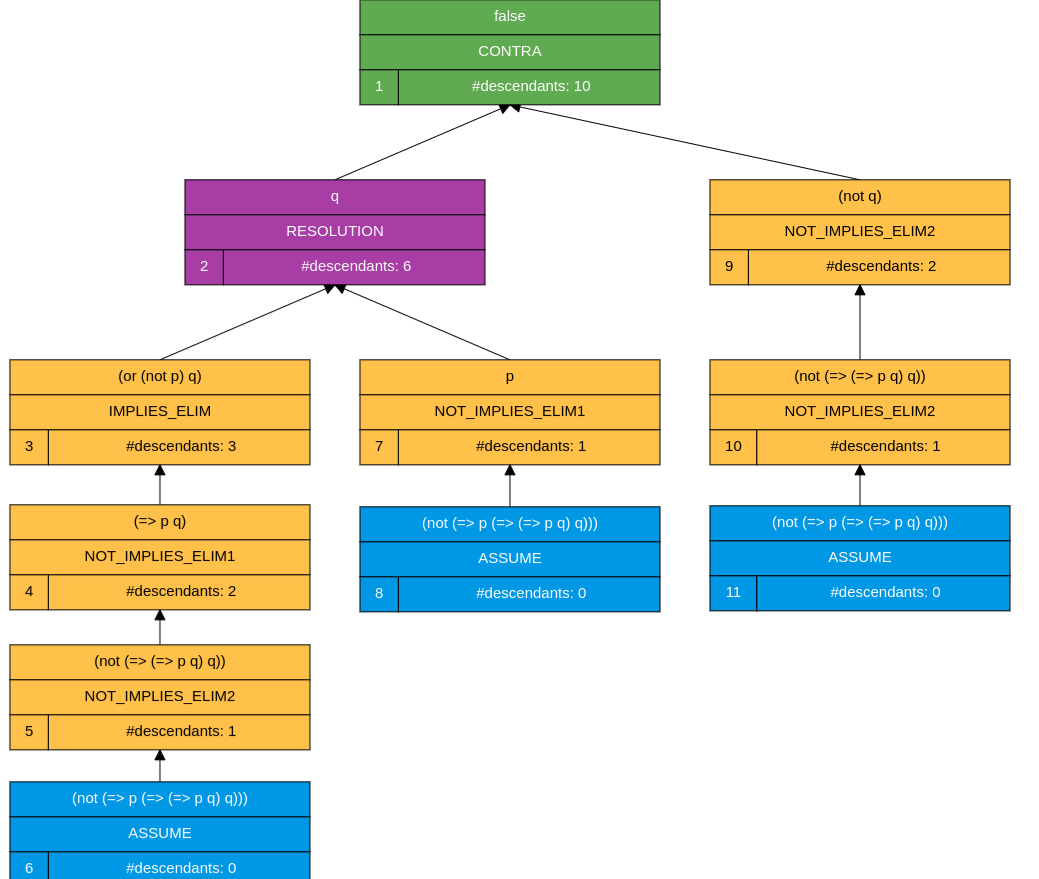
\includegraphics[height=0.8\textheight]{images/mp_cvc5_proof.png}
  \[
    \infer[]{\bot}{\infer[]{q}{\infer[]{\neg p \vee q}{\infer[]{p \rightarrow q}{\infer[]{\neg ((p \rightarrow q) \rightarrow q)}{\neg (p \rightarrow (p \rightarrow q) \rightarrow q)}}} & \infer[]{p}{\neg (p \rightarrow (p \rightarrow q) \rightarrow q)}} & \infer[]{\neg q}{\infer[]{\neg ((p \rightarrow q) \rightarrow q)}{\neg (p \rightarrow (p \rightarrow q) \rightarrow q)}}}
  \]
  \begin{itemize}
    \item Let's encode it in Lean!
  \end{itemize}
\end{frame}

\begin{frame}[fragile]
  \frametitle{Certified Transformations}
  \begin{itemize}
    \item We will use the type below to represent formulas
  \end{itemize}
  \vfill
  \begin{minted}{lean}
  inductive term where
  | const   : Nat -> sort -> term
  | implies : term -> term -> term
  | not     : term -> term
  | top     : term
  | bot     : term
  -- ...
  \end{minted}
\end{frame}

\begin{frame}[fragile]
  \frametitle{Certified Transformations}
  \begin{itemize}
    \item Now the formula representing the negation of modus ponens can be encoded as:
  \end{itemize}
  \vfill
  \begin{minted}{lean}
  def p: term := const 1000 boolSort
  def q: term := const 1001 boolSort

  def notModusPonens: term := not (implies p (implies (implies p q) q))
  \end{minted}
\end{frame}

\begin{frame}
  \frametitle{Certified Transformations}
  \begin{itemize}
    \item Now we need to lift these terms to Props, that is, to expressions that can be proved inside Lean
    \vitem Let's define a function that does that. We can't map terms directly to Props since terms can have free variables, while Props can't, so our function will also receive an \textit{interpretation} for the free variables
    \vitem For now we will only consider terms representing Boolean expressions
  \end{itemize}
\end{frame}

\begin{frame}[fragile]
  \frametitle{Certified Transformations}
  \begin{minted}{lean}
  def Interpretation: Type := Nat -> Prop

  def evalTerm (I : Interpretation) (t : term) : Prop :=
    match t with
    | term.const   i  _  => I i
    | term.not     t1    => Not (evalTerm I t1)
    | term.or      t1 t2 => Or (evalTerm I t1) (evalTerm I t2)
    | term.implies t1 t2 => (evalTerm I t1) -> (evalTerm I t2)
    | term.bot           => False
    | term.top           => True
    | _                  => False
  \end{minted}
\end{frame}

\begin{frame}[fragile]
  \frametitle{Certified Transformations}
  \begin{itemize}
    \item Now we can define what it means for a term to be \textit{satisfied} by a given interpretation:
  \end{itemize}
  \vfill
  \begin{minted}{lean}
  def satisfies (I : Interpretation) (t : term) : Prop :=
    evalTerm I t = True
  \end{minted}
  \vfill
  \begin{itemize}
    \item The rules we have shown before (resolution, congruence, etc.) can now be represented with the following predicate:
  \end{itemize}
  \vfill
  \begin{minted}{lean}
  def impliesIn (t1 t2 : term) : Prop :=
    ∀ (I : Interpretation),
      satisfies I t1 -> satisfies I t2
  \end{minted}
\end{frame}

\begin{frame}[fragile]
  \frametitle{Certified Transformations}
  \begin{itemize}
    \item For instance, the rule \textit{notImplies1}, which states that $\neg (t_{1} \rightarrow t_{2}) \rightarrow t_{1}$, can be encoded in the following way:
  \end{itemize}
  \vfill
  \begin{minted}{lean}
  theorem notImplies1 : ∀ {t1 t2 : term},
    impliesIn (not (implies t1 t2)) t1
  \end{minted}
\end{frame}

\begin{frame}[fragile]
  \frametitle{Certified Transformations}
  \begin{minted}{lean}
  theorem cvc5_th0 : impliesIn notModusPonens bot :=
    fun lean_a0 =>
      have lean_s0 := notImplies2 lean_a0
      have lean_s1 := notImplies1 lean_s0
      have lean_s2 := impliesElim lean_s1
      have lean_s4 := notImplies1 lean_a0
      have lean_s6 := R1 (conjunction lean_s2 lean_s4)
      have lean_s9 := notImplies2 lean_s0
      contradiction (conjunction lean_s9 lean_s6)
  \end{minted}
\end{frame}


\begin{frame}[fragile]
  \frametitle{Certified Transformations}
  \begin{itemize}
    \item Since \texttt{evalTerm I bot} is \texttt{False} for any interpretation \texttt{I}, we can use this to derive:\\ \mintinline{lean}{∀ (I : Interpretation), evalTerm I notModusPonens = False}
    \vitem This result can be used to derive:\\
    \begin{minted}{lean}
    ∀ (I : Interpretation),
      evalTerm I (implies p (implies (implies p q) q)) = True
    \end{minted}
    \vitem Finally, by instantiating the interpretation in a smart way we can prove a theorem \textbf{expressed in Lean's native terms:}
  \end{itemize}
  \vfill
    \begin{minted}{lean}
      ∀ (P Q : Prop), P -> (P -> Q) -> Q
    \end{minted}
\end{frame}

\begin{frame}
  \frametitle{Certified Transformations}
  \begin{itemize}
    \item In order to support more theories, we have to extend our function \texttt{evalTerm} to be able to return values of different types depending on its argument
    \vitem In a language with dependent types, we can achieve this with a \textit{sigma type}
    \vitem If \texttt{T} is a type and \texttt{U} is a type constructor that takes as parameter a value of type \texttt{T}, then \texttt{Sigma T U} is the type of pairs \texttt{⟨t, u⟩} such that \texttt{t} has type \texttt{T} and \texttt{u} has type \texttt{U t}
  \end{itemize}
\end{frame}

\begin{frame}[fragile]
  \frametitle{Certified Transformations}
  \begin{minted}{lean}
  def evalSort : sort → Type := fun s =>
    match s with
    | arrow s1 s2 => evalSort s1 -> evalSort s2
    | boolSort => Prop
    | intSort => Int
    | _ => Prop

  def Interpretation := Nat → @Sigma sort evalSort
  \end{minted}
\end{frame}

\begin{frame}[fragile]
  \frametitle{Certified Transformations}
  \begin{minted}{lean}
  def evalTerm (I : Interpretation) (t : term) :
      Option (@Sigma sort interpSort) :=
    match t with
    | term.const   i  s  => I i
    | term.and     t1 t2 =>
      match evalTerm I t1, evalTerm I t2 with
      | some ⟨ boolSort, p1 ⟩, some ⟨ boolSort , p2 ⟩ =>
          some ⟨ boolSort, And p1 p2 ⟩
      | _,_ => none
    | _ => none
    \end{minted}
\end{frame}

\begin{frame}
  \frametitle{Downsides of Certified Transformations}
  \begin{itemize}
    \item For some rules, it seems too hard to give an explicit proof for the general case
    \begin{itemize}
      \item Resolution
      \item Factor
      \item PermutateClause
    \end{itemize}
    \vitem This approach focuses on \textit{normalizing} terms and Lean is not optimized for that
    \begin{itemize}
      \item For some rules, we have to provide a \textit{proof by reflection} of the well-typedness of the input term
    \end{itemize}
  \end{itemize}
\end{frame}

\section{Reconstructing Proofs with Certifying Transformations}

\begin{frame}
  \frametitle{Certifying Transformations}
  \begin{itemize}
    \item The certifying transformations approach is a well known alternative for these problems
    \vitem The idea is to map the rules into functions that will generate proofs for transformations of terms on the fly
    \vitem The correctness of these proofs will have to be checked every time we use the hammer, as opposed to just once and for all
    \vitem Despite that, our proofs will no longer rely on normalization of terms, so they can potentially be faster
    \vitem Also, it is easier to implement a tactic for a rule than to prove it, as the tactic only cares about a specific case for the rule, while the theorem must consider the most general case
  \end{itemize}
\end{frame}
\begin{frame}
  \frametitle{Certifying Transformations}
  \begin{itemize}
    \item In our case, we will map the rules into tactics. However, we still map rules that are sufficiently simple to theorems
    \vitem We no longer need the \texttt{term} type, as tactics are allowed to inspect the abstract syntax tree of any expression, granting them flexibility
    \vitem We have implemented a library consisting of 75 tactics and theorems that cover all the rules used by cvc5 to reason about formulas involving Booleans, Linear Arithmetic and Equality and Uninterpreted Functions
  \end{itemize}
\end{frame}

\begin{frame}[fragile]
  \frametitle{Certifying Transformations}
  \begin{minted}{lean}
  theorem cvc5_th0 (P Q : Prop) :
      (Not (P → ((P → Q) → Q))) → False :=
    fun lean_a0 : (Not (P → ((P → Q) → Q))) => by
      have lean_s0 : (Not ((P → Q) → Q)) := notImplies2 lean_a0
      have lean_s1 : (P → Q)             := notImplies1 lean_s0
      have lean_s2 : (Or (Not P) Q)      := impliesElim lean_s1
      have lean_s3 : P                   := notImplies1 lean_a0
      have lean_s4 : Q                   := by
        R2 lean_s2, lean_s3, P, [1, 0]
      have lean_s5 : (Not ((P → Q) → Q)) := notImplies2 lean_a0
      have lean_s6 : (Not Q)             := notImplies2 lean_s5
      exact (show False from contradiction lean_s4 lean_s6)
  \end{minted}
\end{frame}

\begin{frame}[fragile]
  \frametitle{PermutateClause Tactic}
  \begin{itemize}
    \item While solving SAT problems, SAT solvers can permutate the order of the terms in a clause. This operation must be justified in proof certificates.
    \vitem This tactic takes as input a permutation and a proof of a clause and outputs a proof for the same clause, with the terms reordered according to the permutation
  \end{itemize}
  \vfill
  \begin{minted}[fontsize=\footnotesize]{lean}
  theorem permutateApp (A B C D E : Prop) : A ∨ B ∨ C ∨ D ∨ E -> E ∨ D ∨ B ∨ C ∨ A :=
    fun h => by permutateClause h, [4, 3, 1, 2, 0]
  \end{minted}
\end{frame}

\begin{frame}[fragile]
  \frametitle{PermutateClause Tactic}
  \begin{minted}{lean}
  def pullProps (props : List Expr) (acc : Expr) (s : Nat) :
      MetaM Expr :=
    match props with
      | [] => return acc
      | e::es => do
          let pulled ← pullCore e acc s
          pullProps es pulled s

  def permutateClauseCore (pf : Expr) (perm : List Nat)
      (s : Nat) : MetaM Expr := do
    let clause : Expr     ← inferType pf
    let props : List Expr ← collectPropsInClause' clause s
    let permutatedProps   := permutateList props (List.reverse perm)
    pullProps permutatedProps pf s
  \end{minted}
\end{frame}

\begin{frame}[fragile]
  \frametitle{Resolution and Factor Tactics}
  \begin{minted}{lean}
  theorem resolutionApp (A B C D : Prop) :
      A ∨ B ∨ C -> D ∨ ¬ B -> A ∨ C ∨ D := by
    intros h₁ h₂
    R1 h₁, h₂, B

  theorem factorApp (A B C : Prop) :
      A ∨ B ∨ A ∨ A ∨ B ∨ C ∨ B → A ∨ B ∨ C := by
    intro h
    factor h
  \end{minted}
\end{frame}

\begin{frame}[fragile]
  \frametitle{SumBounds Tactic}
  \begin{minted}{lean}
  theorem sumBoundsApp (a c : Nat) (b d : Int) (e f : Rat) :
      a < d -> b ≤ e -> c ≤ f -> a + (b + c) < d + (e + f) := by
    intros h₁ h₂ h₃
    sumBounds [h₁, h₂, h₃]
  \end{minted}
\end{frame}

% \begin{frame}[fragile]
%   \frametitle{Congruence}
% \end{frame}



\section{Demo: Proof Checking}

\begin{frame}[fragile]
  \frametitle{Lean-SMT}
  \begin{minted}[fontsize=\footnotesize]{lean}
  import Smt

  variable {G : Type} [Nonempty G] (op : G -> G -> G) (inv : G -> G) (e : G)

  axiom assoc : ∀ a b c, op a (op b c) = op (op a b) c
  axiom inverse : ∀ a, op (inv a) a = e
  axiom ident : ∀ a, op e a = a

  theorem inverse' : ∀ a, op a (inv a) = e := by
    smt [assoc op, inverse op inv e, ident op e]

  theorem identity' : ∀ a, op a e = a := by
    smt [assoc op, inverse op inv e, ident op e, inverse' op inv e]

  theorem unique_identity : ∀ e', (∀ z, op e' z = z) -> e' = e := by
    smt [assoc op, inverse op inv e, ident op e]

  -- Credits also to Abdalrhman Mohammed, Cesare Tinelli and Wojciech Nawrocki
  \end{minted}
\end{frame}

\begin{frame}
  \frametitle{Evaluation}
  \begin{itemize}
    \item We used a test set of 6102 SMT problems provided by SMT-LIB, containing only problems expressed in the theories we support
    \vitem After producing Lean scripts for these problems with cvc5, we filtered out proofs whose size was bigger than 1mb, resulting in 877 proofs
    \vitem We ran our checker on these 877 proofs. Lean accepted 281 of these proofs
  \end{itemize}
\end{frame}

\begin{frame}
  \frametitle{Evaluation}
  \begin{itemize}
    \item 302 failed for exceeding Lean's resources
    \vitem 106 failed for cvc5 misinterpreting some Lean operator
    \vitem 11 failed for a bug in an implementation of a tactic (which was fixed)
    \vitem We are in the process of understanding why the other 182 failed
  \end{itemize}
\end{frame}

\section{Thank you! Questions?}

% \section{Demo: Lean-SMT}

% \maketitle

\end{document}

%%% Local Variables:
%%% mode: latex
%%% TeX-master: t
%%% End:
